\documentclass[12pt]{article}
\usepackage{helvet}
\usepackage{graphicx}
\usepackage{geometry}
\geometry{
    a4paper,
    top = 2cm,
    left = 2cm,
    right = 2cm,
    bottom = 3cm
}
\usepackage[utf8]{inputenc}
\usepackage[spanish,mexico]{babel} % Renombra en automático los elementos a español
\addto\captionsspanish{
  \renewcommand{\figurename}{Imagen}
  \renewcommand{\tablename}{Tabla}
}
\usepackage{float}  % Etiqueta 'H' (mayus) en figuras (imágenes)
\usepackage{array}  % Padding en tablas
\usepackage{tabularx}
\usepackage{url}    % Etiqueta url en .bib
\usepackage{booktabs}   % Manejo de caudros (tablas)
\usepackage[T1]{fontenc}    % Codificación de fuentes
\usepackage[autostyle, spanish=mexican]{csquotes}       % Paquete para comillas tipográficas
\usepackage{comment}    % Comentar bloques de líneas mediante begin-end
\usepackage{multicol}   % Para poner contenido a doble columna
\usepackage{enumitem}   % Para utilizar [noitemsep, topsep=0pt] en itemize
\usepackage{amsmath}
\usepackage{mathabx} % Para testar en math mode
\usepackage{comment}
\usepackage{longtable}
\usepackage[hidelinks]{hyperref}
\usepackage{caption}
\usepackage[
  backend=biber,
  style=apa,
  sorting=nyt
]{biblatex}
\DeclareLanguageMapping{spanish}{spanish-apa}
\renewcommand{\familydefault}{\sfdefault}
\newenvironment{localsubgroup}
  {$\left\{\tabular{l}}
  {\endtabular\right.$}


\addbibresource{bibliography/p05.bib}

\begin{comment}
Indicaciones del profesor:
Máquina Virtual Windows Sever 2008 R2

Se debe crear uan máquina virtual utilizando Windows 200X Server y se le deberán instalar los siguientes servicios:
- Directorio Activo
- DNS
- Servicios de Archivos y Almacenamiento
- Servidor de Aplicaciones

Consideraciones:
- Carpeta a compartir: SoftwareRed
- Usuario: clientewin
- Contraseña: so123&
- Grupo de trabajo: Sistemas

El cliente debe ser la máquina nativa y se debe trabajar con la opción de puente en red de la MV para poder establecer comunicación.

Rango de páginas exigido: mínimo 18 páginas, máximo 40 páginas. Objetivo: 27 páginas.

Índice aprobado y presupuesto de páginas (reajustado tras la redacción completa y la pasada de compresión sobre la prosa de las secciones 1 a 8; las cifras son las páginas reales que rinden en el PDF compilado):
1. Entorno de virtualización [5.0 págs. | Acum: 5.0]
   1.1. Hipervisor de tipo 2 y máquina invitado
   1.2. Hardware virtual, firmware y disco de la MV
   1.3. Red en modo puente sobre la LAN física
2. Instalación de Windows Server 2008 R2 [3.0 págs. | Acum: 8.0]
   2.1. Requisitos de hardware, CPU, ediciones disponibles
   2.2. Despliegue de la instalación y opciones de arranque
   2.3. Tareas de configuración inicial y preparación del sistema
3. Arquitectura interna del servidor [4.0 págs. | Acum: 12.0]
   3.1. Núcleo NT: modo kernel, modo usuario y API nativa
   3.2. Ejecutivo, gestor de objetos y gestor de E/S
   3.3. NTFS: MFT, journaling y metadatos
4. Directorio Activo [4.0 págs. | Acum: 16.0]
   4.1. Modelo de dominio: objetos, contenedores, atributos y bosque
   4.2. Rol AD DS y promoción del controlador de dominio
   4.3. Unidades organizativas, cuentas, grupos y objetos de política de grupo
5. Servicio DNS [3.0 págs. | Acum: 19.0]
   5.1. Estructura del servicio, zonas y tipos de registros
   5.2. Integración con AD DS y resolución de nombres del servidor
6. Servicios de archivos y almacenamiento [4.0 págs. | Acum: 23.0]
   6.1. Rol File Services: recursos compartidos, cuotas y DFS
   6.2. Carpeta compartida SoftwareRed: permisos de uso frente a NTFS
   6.3. Administración de archivos compartidos y MMC
7. Servidor de aplicaciones e IIS 7.5 [3.0 págs. | Acum: 26.0]
   7.1. Rol Application Server: COM+, MS DTC, WCF
   7.2. IIS 7.5: arquitectura modular, application pools y módulos
   7.3. Publicación del sitio, enlace de puerto y prueba HTTP
8. Cliente nativo e integración [1.3 págs. | Acum: 27.3]
   8.1. Configuración del cliente en el grupo de trabajo Sistemas
   8.2. Cuenta clientewin y montaje del recurso compartido
   8.3. Batería de verificación de los cuatro servicios
9. Conclusiones [2.0 págs. | Acum: 29.3]
\end{comment}

\begin{document}
\pagenumbering{roman}

\begin{titlepage}
  \thispagestyle{empty}
  \newgeometry{left = 1cm, right = 1cm, top = 1cm, bottom = 2cm}

  \noindent
  \begin{minipage}[c]{3.5cm}
    
\includegraphics[width=3.5cm]{media/titlepage/Escudo-UNAM.pdf}
  \end{minipage}\hfill
  \begin{minipage}[c][3.5cm][c]{\dimexpr\textwidth-7cm\relax}
    \centering
    {\large\textbf{Universidad Nacional Autónoma de México}\\[0.6em] 
    \Large\textbf{Facultad de Ingeniería}\\[0.6em]
    \large Sistemas Operativos}
  \end{minipage}\hfill
  \begin{minipage}[c]{3.5cm}
    \raggedleft
    
\includegraphics[width=3.5cm]{media/titlepage/FI.png}
  \end{minipage}
\centering\huge
  \vfill
    Grupo 1 \\
    Ing. Angel Isidro Mercado
  \vfill
    \textbf{Proyecto 5. Windows Server IIS}
  \vfill\large
    320304435 - Cabrera Rojas Oscar
  \vfill

  \noindent\footnotesize \hfill Ciudad Universitaria, CDMX a 09 de noviembre del 2026
\end{titlepage}
\restoregeometry

\tableofcontents

\newpage
\pagenumbering{arabic}
\setcounter{page}{1}

\section{Entorno de virtualización}
\label{sec:entornoVirtualizacion}

\subsection{Hipervisor de tipo 2 y máquina invitado}
\label{sec:hipervisorTipo2}

El servidor que concentra los cuatro servicios de este proyecto no se instala sobre hardware propio, sino como sistema operativo invitado dentro de una máquina virtual (MV) creada sobre la computadora que actuará además como cliente. El software que hace posible esa abstracción es el monitor de máquina virtual, conocido como \textit{hypervisor}: abstrae los recursos físicos —procesador, memoria, red y almacenamiento— para que sobre un mismo anfitrión se ejecuten pilas de cómputo independientes.

La distinción operativa que interesa aquí separa dos familias de hypervisor. El de tipo 1 se carga como una capa de software directamente sobre el servidor físico y controla por sí mismo los recursos reales de la máquina, sin que exista un sistema operativo intermediario; sus representantes son VMware ESXi, Microsoft Hyper-V y las variantes de Xen \parencite[\S 14.2, p.\ 633]{stallings2018operating}. El de tipo 2, en cambio, explota los recursos y las funciones del sistema operativo anfitrión y se ejecuta como un módulo de software sobre él, delegando en ese sistema operativo la totalidad de las interacciones con el hardware; los representantes más conocidos son VMware Workstation y Oracle VM VirtualBox \parencite[\S 14.2, p.\ 633]{stallings2018operating}.

La Tabla~\ref{tab:comparativaHipervisores} contrapone ambas familias en los ejes que condicionan la elección. El hipervisor de tipo 2 ofrece mejor desempeño general, porque no compite por los recursos con un sistema operativo completo que se ejecuta por debajo, y ofrece mayor aislamiento, ya que las peticiones de recursos de cada MV se atienden fuera de la propia MV y no pueden afectar a las demás ni al hipervisor que las sostiene \parencite[\S 14.2, p.\ 633]{stallings2018operating}. A cambio, el tipo 2 es el que permite a un administrador llevar un entorno aislado sin dedicar un servidor completo a esa función, conservando además el espacio de trabajo del sistema operativo anfitrión, condición que hace viable alojar en el mismo equipo el servidor del proyecto y el cliente nativo que lo consume.

\begin{table}[htbp]
\centering
\small
\renewcommand{\arraystretch}{1.15}
\renewcommand{\tabularxcolumn}[1]{m{#1}}
\setlength{\emergencystretch}{1.5em}
\caption{Comparativa técnica entre los dos tipos de hipervisor.}
\label{tab:comparativaHipervisores}
\begin{tabularx}{\textwidth}{>{\centering\arraybackslash}m{3.2cm} X X}
\toprule
\textbf{Criterio} & \textbf{Hipervisor de tipo 1} & \textbf{Hipervisor de tipo 2} \\
\midrule
\textbf{Relación con el sistema operativo anfitrión} & Se carga directamente sobre el servidor físico, sin sistema operativo por debajo, y controla por sí mismo los recursos reales de la máquina. & Se ejecuta como módulo sobre el sistema operativo anfitrión, que administra el hardware en nombre del hipervisor y resuelve por él todas las interacciones. \\
\addlinespace
\textbf{Desempeño} & Mayor: no compite por los recursos con un sistema operativo completo, por lo que admite más MV por servidor. & Menor: existe una capa adicional de software entre la MV y el dispositivo físico. \\
\addlinespace
\textbf{Aislamiento y seguridad} & Las MV solicitan recursos que se resuelven fuera de ellas; una MV maliciosa no alcanza a afectar a las demás ni al hipervisor. & El aislamiento no ofrece la misma garantía, pues una MV comprometida puede influenciar sobre el contexto del anfitrión. \\
\addlinespace
\textbf{Representantes} & VMware ESXi, Microsoft Hyper-V, variantes de Xen. & VMware Workstation, Oracle VM VirtualBox. \\
\addlinespace
\textbf{Aplicación en este proyecto} & Exige un servidor dedicado a la función de virtualización. & Se instala sobre la computadora cliente y permite conservar el sistema operativo nativo en operación. \\
\bottomrule
\end{tabularx}
\end{table}

El comportamiento del hypervisor hacia la MV tiene una consecuencia medible en el diseño de la máquina invitada. Cuando el sistema operativo invitado ejecuta una instrucción privilegiada que un sistema nativo ejecutaría directamente sobre su hardware, esa instrucción es interceptada por el hipervisor, que la resuelve en nombre de la MV; ese mecanismo de intercepción y traducción de entrada/salida (E/S) introduce una penalización de desempeño que las mejoras de hardware y de software han ido reduciendo \parencite[\S 14.2, p.\ 631]{stallings2018operating}. Sobre ese mecanismo actúan las extensiones de virtualización asistida por hardware, AMD-V de Advanced Micro Devices y VT-x de Intel, esta última con un conjunto de instrucciones denominado Virtual Machine Extensions (VMX); cuando están presentes en el procesador anfitrión, el hipervisor deja de mantener esas funciones en su propio código y las operaciones se ejecutan íntegramente dentro del procesador, lo que permite un código más pequeño y eficiente sin exigir modificación alguna del sistema operativo invitado, a diferencia de la paravirtualización \parencite[\S 14.2, p.\ 635]{stallings2018operating}.

La unidad de virtualización completa tiene, además, una naturaleza peculiar: una MV es un conjunto de archivos. El archivo de configuración describe sus atributos ---cuántos procesadores virtuales se le asignan, cuánta memoria aleatoria (RAM) dispone, a qué dispositivos de E/S tiene acceso, cuántas interfaces de red presenta y qué almacenamiento ve---, y ese almacenamiento se materializa casi siempre como discos virtuales que son archivos adicionales en el sistema de archivos del anfitrión; al encender la MV se crean además archivos de registro y de paginación \parencite[\S 14.2, p.\ 632]{stallings2018operating}. Esta representación en archivos explica dos propiedades que el despliegue aprovecha: la posibilidad de copiar el conjunto para obtener un respaldo íntegro y la aparición de las plantillas como mecanismo de aprovisionamiento rápido.

\subsection{Hardware virtual, firmware y disco de la MV}
\label{sec:hardwareVirtual}

El \textit{firmware} que arranca la MV no es el del anfitrión sino uno propio, y su inicialización opera sobre los dispositivos virtuales que el hipervisor expone. El resultado es que la MV se presenta ante su propio sistema operativo como un equipo con una configuración de hardware definida y cerrada, y no como una ventana hacia la máquina que la hospeda. Toda la E/S que el invitado emite hacia sus periféricos virtuales recorre una ruta con dos etapas: primero el controlador del dispositivo dentro de la MV, que se comunica con un dispositivo emulado y no real; después, la pila de E/S del hipervisor, que traduce las direcciones de E/S del invitado a las direcciones del host y encamina la petición hacia el controlador del dispositivo físico real \parencite[\S 14.6, p.\ 646]{stallings2018operating}. La Tabla~\ref{tab:rutaIoVirtualizada} detalía cada eslabón de ese trayecto, con el efecto que introduce sobre el sistema invitado.

\begin{table}[htbp]
\centering
\small
\renewcommand{\arraystretch}{1.15}
\renewcommand{\tabularxcolumn}[1]{m{#1}}
\setlength{\emergencystretch}{1.5em}
\caption{Eslabones de la ruta de entrada/salida de una máquina virtual con adaptador de red emulado.}
\label{tab:rutaIoVirtualizada}
\begin{tabularx}{\textwidth}{>{\centering\arraybackslash}m{3.4cm} X}
\toprule
\textbf{Eslabón} & \textbf{Comportamiento y efecto sobre el sistema invitado} \\
\midrule
\textbf{Controlador en la MV} & El controlador de red de la MV opera como lo haría sobre una tarjeta física, sin conocer que el dispositivo es emulado; el invitado usa el mismo controlador y la misma pila de protocolos que en una máquina real. \\
\addlinespace
\textbf{Dispositivo emulado} & Dispositivo genérico implementado por el hipervisor, del tipo Intel \texttt{e1000} en el caso de la red; el invitado ve una interfaz con dirección de control de acceso al medio (MAC) propia y con las capacidades declaradas por el emulador. \\
\addlinespace
\textbf{Pila de E/S del hipervisor} & Traduce las direcciones de E/S del invitado a las del anfitrión y enruta cada petición al dispositivo físico correcto, manteniendo el aislamiento entre MV en el punto de acceso al hardware compartido. \\
\addlinespace
\textbf{Controlador del host} & El controlador real, asociado a la tarjeta física del anfitrión, ejecuta la operación sobre el dispositivo real, de modo que el tráfico sale a la red física con la identidad de la MV y no con la del anfitrión. \\
\bottomrule
\end{tabularx}
\end{table}

Los recursos asignados a la MV no son arbitrarios: el sistema operativo invitado debe recibir una configuración que satisfaga los requisitos del producto, que se detallan en la sección de instalación y que la Tabla~\ref{tab:parametrosMaquinaVirtual} translate a valores concretos. La memoria disponible condiciona además el dimensionamiento del sistema de archivos, porque los equipos con más de 16 GB de RAM requieren espacio adicional para los archivos de paginación, hibernación y vuelco de memoria \parencite{microsoftInstallWs2008r2}; la partición del sistema se dimensiona por tanto por encima del mínimo absoluto con un margen que absorbe el crecimiento de la base de datos del directorio, los registros del servicio de nombres de dominio (DNS) y los archivos publicados.

\begin{table}[htbp]
\centering
\small
\renewcommand{\arraystretch}{1.15}
\renewcommand{\tabularxcolumn}[1]{m{#1}}
\setlength{\emergencystretch}{1.5em}
\caption{Parámetros de la máquina virtual y justificación de su asignación.}
\label{tab:parametrosMaquinaVirtual}
\begin{tabularx}{\textwidth}{>{\centering\arraybackslash}m{3.6cm} X X}
\toprule
\textbf{Parámetro} & \textbf{Valor asignado} & \textbf{Criterio de asignación} \\
\midrule
\textbf{Firmware invitado} & BIOS o firmware de interfaz extensible (EFI), según el modelo de hardware elegido para la MV. & La MV arranca su propio firmware sobre los dispositivos emulados; el firmware del anfitrión no interviene. \\
\addlinespace
\textbf{Procesadores virtuales} & Dos. & Cubre la carga de los servicios previstos sin forzar el plan de unidad central de procesamiento (CPU) del anfitrión. \\
\addlinespace
\textbf{Memoria RAM} & 4 GB. & Supera con holgura los 2 GB recomendados por el fabricante y deja margen para las cachés de base de datos y el crecimiento de los servicios. \\
\addlinespace
\textbf{Disco virtual} & Archivo de 60 GB con aprovisionamiento dinámico sobre el sistema de archivos del anfitrión. & Cubre los 40 GB recomendados y absorbe la expansión de la base de datos del directorio, los registros del servicio de nombres de dominio (DNS) y los archivos publicados. \\
\addlinespace
\textbf{Adaptador de red} & Una interfaz emulada en modo puente, con dirección propia dentro de la red física. & Permite que la MV participe en la red local con identidad propia, condición para el diálogo con el cliente nativo. \\
\addlinespace
\textbf{Tarjeta de video} & Memoria emulada suficiente para 1024$\times$768. & Cubre la resolución mínima de 800$\times$600 exigida por la instalación. \\
\bottomrule
\end{tabularx}
\end{table}

\subsection{Red en modo puente sobre la LAN física}
\label{sec:puenteRed}

La condición de comunicación entre el servidor y el cliente no se satisface con cualquier modo de red virtual. En el modo de traducción de direcciones de red (NAT, Network Address Translation), que es la configuración que el asistente de creación de MV selecciona por omisión, la MV no posee dirección propia en la red externa: se levanta una red privada en el anfitrión y la MV obtiene en ella una dirección del servidor de configuración dinámica de direcciones (DHCP) virtual, de modo que ambas comparten una identidad de red única e invisible desde el exterior \parencite[p.\ 147]{vmwareWorkstationPro26h1}. El modo de red aislada crea un segmento contenido por completo dentro del anfitrión \parencite[p.\ 147]{vmwareWorkstationPro26h1}. Ninguno de los dos permite que el cliente nativo abra sesiones contra el servidor por la red física.

El modo puente resuelve el problema por el otro extremo: el adaptador de red virtual de la MV se conecta a un adaptador de red físico del anfitrión, y ese adaptador físico da a la MV acceso a la red de área local (LAN) que utiliza el anfitrión, con adaptadores alámbricos o inalámbricos \parencite[p.\ 150]{vmwareWorkstationPro26h1}. La diferencia decisiva es de identidad: en el modo puente la MV se configura como un interlocutor único y propio en la red, separado del sistema anfitrión, participa de ella como cualquier otro equipo y las demás máquinas pueden contactarla como si fuera una computadora física \parencite[p.\ 150]{vmwareWorkstationPro26h1}. La Img.~\ref{fig:puenteRedVmnet0} esquematiza el trayecto del enlace.

\begin{figure}[htbp]
    \centering
    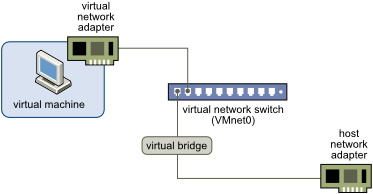
\includegraphics[width=0.72\columnwidth]{media/p05/puenteRedVmnet0.png}
    \caption{Conexión de la máquina virtual a la red física a través del adaptador del anfitrión en modo puente \parencite[p.\ 151]{vmwareWorkstationPro26h1}.}
    \label{fig:puenteRedVmnet0}
\end{figure}

Al quedar la MV y el cliente nativo en el mismo segmento de la red física, la comunicación deja de depender de mecanismos de traducción o de reenvío de puertos y se apoya en sesiones TCP ---Transmission Control Protocol--- directas iniciadas por el cliente. Los servicios que se activarán en los capítulos siguientes quedan alcanzables por esa vía: el acceso a recursos compartidos sobre el puerto 445, la resolución de nombres sobre el 53, la autenticación de dominio sobre el 88 y las consultas de directorio sobre el 389 y el 636, además del tráfico HTTP sobre los puertos 80 y 443 una vez publicado el sitio.

La configuración del puente exige definir dos niveles distintos que con frecuencia se confunden. El primero corresponde al conmutador virtual VMnet0, que se crea durante la instalación de la aplicación de virtualización y cuyo destino puede fijarse desde el editor de redes virtuales; por omisión opera en modo de puente automático y se enlaza con todos los adaptadores activos del anfitrión, y en un equipo que cuenta con interfaz inalámbrica y con cable, o con adaptadores virtuales de otros hypervisors instalados, esa selección automática puede apuntar al dispositivo equivocado \parencite[p.\ 152]{vmwareWorkstationPro26h1}. Fijar VMnet0 explícitamente sobre el adaptador físico en uso requiere privilegios de administrador en el caso de un anfitrión con Windows \parencite[p.\ 151]{vmwareWorkstationPro26h1}. El segundo nivel corresponde al adaptador de la propia MV, que dentro de la configuración de la máquina debe establecerse en modo puente \parencite[p.\ 149]{vmwareWorkstationPro26h1}.

Una vez establecido el enlace, la MV necesita su propia dirección en la red, igual que cualquier equipo de la LAN, y la obtiene del servidor DHCP de la red física o mediante una asignación estática definida dentro del sistema invitado \parencite[p.\ 151]{vmwareWorkstationPro26h1}. Esta dirección es la que el cliente nativo utiliza como destino de sus conexiones, y es también la que el servicio DNS del servidor registrará para su propio nombre, de modo que el nombre y la dirección del servidor puedan resolverse desde la red sin depender de la tabla de nombres del anfitrión.

\section{Instalación de Windows Server 2008 R2}
\label{sec:instalacionWindowsServer}

\subsection{Requisitos de hardware, CPU, ediciones disponibles}
\label{sec:requisitosHardware}

El dimensionamiento de la instalación se apoya en los requisitos estimados que el fabricante publica para el producto, que varían según la configuración del equipo y las aplicaciones instaladas \parencite{microsoftInstallWs2008r2}: un procesador de 64 bits de 1.4 GHz como mínimo, un mínimo de 512 MB de memoria con un máximo de 32 GB en la edición Standard y de 2 TB en las ediciones Enterprise, Datacenter y para Itanium, y un mínimo absoluto de 32 GB para la partición del sistema, valor que debe ampliarse por la instalación sobre red, por los archivos de paginación, hibernación y vuelco de memoria en equipos con más de 16 GB de RAM y por el crecimiento sostenido de la partición a medida que se aplican actualizaciones \parencite{microsoftInstallWs2008r2}. Entre los demás requisitos figuran una unidad de disco de video digital (DVD), un monitor Super VGA de 800$\times$600 o de mayor resolución, teclado y ratón, y acceso a Internet \parencite{microsoftInstallWs2008r2}.

Dos restricciones de la plataforma condicionan el resto del diseño. La primera es la exclusividad de la arquitectura de 64 bits: todas las ediciones de Windows Server 2008 R2 son únicamente de 64 bits y las actualizaciones in situ desde sistemas de 32 bits no están admitidas \parencite{microsoftInstallWs2008r2}. La segunda es la exigencia de firma digital para los controladores en modo kernel: en las versiones x64 un controlador no firmado no se carga, y la única vía para habilitarlo consiste en reiniciar, pulsar F8 y seleccionar Deshabilitar aplicación de firma de controlador \parencite{microsoftInstallWs2008r2}. La condición incide sobre la máquina virtual, cuyos adaptadores de red y de almacenamiento son dispositivos emulados a los que el sistema operativo debe asociar un controlador.

El catálogo de la plataforma incluye los cinco roles de servidor que requiere este despliegue: Directorio Activo (AD DS), DNS Server, File Services, Application Server y Web Server (IIS) \parencite{microsoftServerRoles}, y la Tabla~\ref{tab:edicionesWindowsServer} contrasta las ediciones con el papel que cada una juega en el proyecto. Conviene registrar que el producto utilizado es una plataforma cuyo ciclo de vida ha concluido: el soporte principal de Windows Server 2008 R2 terminó el 14 de enero de 2015 y el extendido el 15 de enero de 2020 \parencite{microsoftLifecycleWs2008r2}. El despliegue responde por tanto a un requisito de formación sobre una arquitectura concreta y no constituye una recomendación de producto, y la misma estructura conceptual ---directorio, nombres, archivos y servidor de aplicaciones--- se sostiene hoy sobre versiones posteriores que difieren en el empaquetado de los roles y en la superficie de administración, pero no en los principios aquí trazados.

\begin{table}[htbp]
\centering
\small
\renewcommand{\arraystretch}{1.15}
\renewcommand{\tabularxcolumn}[1]{m{#1}}
\setlength{\emergencystretch}{1.5em}
\caption{Ediciones de Windows Server 2008 R2 y encaje en el despliegue.}
\label{tab:edicionesWindowsServer}
\begin{tabularx}{\textwidth}{>{\centering\arraybackslash}m{3.0cm} X X}
\toprule
\textbf{Edición} & \textbf{Rasgo que la distingue} & \textbf{Encaje en el proyecto} \\
\midrule
\textbf{Standard} & Tope de 32 GB de RAM y catálogo completo de roles. & \textbf{Adoptada}: los cinco roles requeridos se instalan sin rebasar el límite de memoria ni el mínimo de 32 GB de disco. \\
\addlinespace
\textbf{Enterprise} & Tope de 2 TB de RAM. & No aporta capacidad: el alcance funcional es el de un servidor de grupo de trabajo. \\
\addlinespace
\textbf{Datacenter} & Tope de 2 TB de RAM; cargas consolidadas a escala de centro de datos. & Excede el alcance del proyecto en función y en capacidad. \\
\addlinespace
\textbf{Web Server} & Publicación web; una de las cuatro ediciones principales del producto \parencite{microsoftInstallWinServer2008}. & No se ajusta: el despliegue exige además el directorio, los archivos y el servidor de aplicaciones, y el rol Application Server no está disponible en esta edición \parencite{microsoftApplicationServerRole}. \\
\bottomrule
\end{tabularx}
\end{table}

\subsection{Despliegue de la instalación y opciones de arranque}
\label{sec:opcionesInstalacion}

El programa de instalación trabaja en varias etapas: solicita información básica, copia los archivos, reinicia el equipo y concluye presentando el menú de tareas de configuración inicial \parencite{microsoftInstallWs2008r2}. La secuencia y sus decisiones asociadas quedan resumidas en el cuadro sinóptico de la Figura~\ref{fig:etapasInstalacion}.

\begin{figure}[htbp]
\centering
\begin{minipage}{0.9\textwidth}
\begin{localsubgroup}
Etapas de la instalación
\begin{localsubgroup}
- Información básica \\
- Copia de archivos y reinicio \\
- Tareas de configuración inicial
\end{localsubgroup}
\end{localsubgroup}
\end{minipage}
\caption{Secuencia de etapas del programa de instalación de Windows Server 2008 R2 \parencite{microsoftInstallWs2008r2}.}
\label{fig:etapasInstalacion}
\end{figure}

La decisión de mayor alcance es la del tipo de instalación. La instalación completa (\textit{Full installation}) incorpora la interfaz gráfica de escritorio, mientras que \textit{Server Core} constituye una instalación mínima del sistema operativo en la que no se instala la interfaz tradicional de Windows y el servidor debe configurarse desde la línea de comandos; además, con esta variante no pueden instalarse algunos módulos que dependen de .NET Framework o de código administrado \parencite{microsoftInstallWinServer2008}. La propia documentación matiza esa limitación: con la incorporación de .NET Framework a Server Core en Windows Server 2008 R2, la variante resulta más atractiva para quien se dedique a alojar aplicaciones \parencite{microsoftInstallWinServer2008}. Las rutas de actualización admitidas confirman que cada edición existe en ambas formas y que las actualizaciones in situ se circunscriben a la misma variante \parencite{microsoftInstallWs2008r2}.

El despliegue opta por la instalación completa. La razón es operativa y no de recursos: la incorporación de los cuatro servicios se realiza con el asistente de instalación de roles y características de \textit{Server Manager} \parencite{microsoftServerRoles}, y su administración posterior exige las consolas de administración gráfica de cada servicio, que no existen en Server Core. La Figura~\ref{fig:opcionServerCore} muestra la pantalla de selección de edición, donde conviven las dos variantes de instalación.

\begin{figure}[htbp]
    \centering
    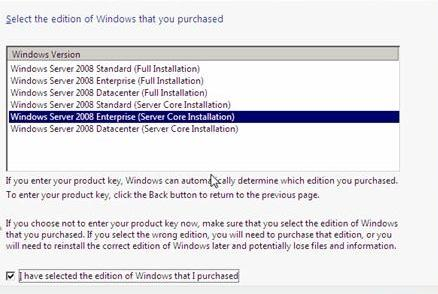
\includegraphics[width=0.75\columnwidth]{media/p05/opcionServerCore.jpg}
    \caption{Pantalla de selección de edición, con las variantes de instalación completa y Server Core para cada edición \parencite{microsoftInstallWinServer2008}.}
    \label{fig:opcionServerCore}
\end{figure}

La partición de destino se elige en una pantalla que muestra los volúmenes detectados con su tamaño total y su espacio libre, y que ofrece la carga de controladores de almacenamiento mediante la tecla F6 \parencite{microsoftInstallWs2008r2}.

\subsection{Tareas de configuración inicial y preparación del sistema}
\label{sec:tareasIniciales}

Al iniciar sesión por primera vez se abre de forma automática la ventana de tareas de configuración inicial, cuyos comandos permiten ajustar el servidor a las necesidades del caso \parencite{microsoftInstallWinServer2008}. El catálogo de esas tareas abarca la contraseña y la identidad del administrador, la pertenencia a un dominio o grupo de trabajo, el nombre del equipo, el escritorio remoto, Windows Update y el Firewall de Windows; la Tabla~\ref{tab:tareasIniciales} contrasta el valor por omisión de cada una con el que adopta el despliegue.

\begin{table}[htbp]
\centering
\small
\renewcommand{\arraystretch}{1.15}
\renewcommand{\tabularxcolumn}[1]{m{#1}}
\setlength{\emergencystretch}{1.5em}
\caption{Tareas de configuración inicial: valor por omisión y valor aplicado.}
\label{tab:tareasIniciales}
\begin{tabularx}{\textwidth}{>{\centering\arraybackslash}m{3.4cm} m{3.0cm} X}
\toprule
\textbf{Tarea} & \textbf{Valor por omisión} & \textbf{Valor aplicado y fundamento} \\
\midrule
\textbf{Contraseña de administrador} & Vacía. & Se establece una contraseña no vacía, requisito mínimo para exponer el servidor a la red física en modo puente. \\
\addlinespace
\textbf{Grupo de trabajo o dominio} & \textit{WORKGROUP}. & Se une al grupo de trabajo \textit{Sistemas}, que es el mismo al que pertenece la máquina nativa que actúa como cliente. \\
\addlinespace
\textbf{Nombre del equipo} & Generado al azar. & Nombre estable y predecible, necesario para resolverlo desde el cliente y para registrarlo en el servicio DNS. \\
\addlinespace
\textbf{Windows Update} & Desactivado. & Se activa y se aplican las actualizaciones antes de la promoción del servidor a controlador de dominio. \\
\addlinespace
\textbf{Firewall de Windows} & Activado. & Se mantiene activo; la instalación de cada rol incorpora sus reglas de entrada correspondientes. \\
\addlinespace
\textbf{Escritorio remoto} & Desactivado. & Se habilita para la administración del servidor desde el cliente, una vez estabilizado el acceso. \\
\bottomrule
\end{tabularx}
\end{table}

Dos de esos valores por omisión tienen consecuencias que exceden la configuración inmediata. El grupo de trabajo por omisión es WORKGROUP y no el nombre requerido, de modo que la primera tarea sustantiva consiste en incorporar el servidor al grupo de trabajo Sistemas: desde ese instante el servidor y el cliente nativo son pares dentro del mismo grupo y pueden resolverse mutuamente por \textit{NetBIOS}, condición que permite validar el recurso compartido antes de que exista el dominio. Esta pertenencia al grupo de trabajo es, sin embargo, transitoria: en cuanto el servidor se promueva a controlador de dominio, abandonará el grupo de trabajo y quedará integrado en el dominio que se cree en la sección del directorio activo, y el cliente dejará de autenticar sus sesiones contra él de forma transparente \parencite{microsoftInstallADDS}.

La segunda consecuencia se relaciona con el cortafuegos: las aplicaciones de servidor que deben recibir conexiones entrantes no funcionan hasta que se crean reglas de entrada que las autoricen \parencite{microsoftInstallWs2008r2}. El despliegue deja el cortafuegos activo y confía en que la incorporación de cada rol incorpore las reglas de permisos de programa que ese rol requiere, de manera que la superficie expuesta quede acotada a los puertos que cada servicio necesita y no a un permiso general sobre el sistema.

La preparación del entorno de directorio con las actualizaciones del producto solo tiene lugar cuando el servidor se incorpora a un bosque de Active Directory ya existente, caso en el que debe ejecutarse la utilidad \textit{Adprep.exe} sobre los controladores de dominio vigentes antes de instalar el rol de directorio \parencite{microsoftInstallWs2008r2}. Como aquí el bosque se crea desde cero, no existe dominio ni bosque que preparar y la etapa se reduce a mantener el sistema actualizado antes de la promoción.

\section{Arquitectura interna del servidor}
\label{sec:arquitecturaInterna}

\subsection{Núcleo NT: modo kernel, modo usuario y API nativa}
\label{sec:nucleoNt}

Windows Server 2008 R2 deriva del linaje Windows NT, y su arquitectura conserva la organización en capas que ese linaje introdujo: cada capa se compone de varios módulos relativamente simples con una funcionalidad muy específica \parencite[\S 12.3, p.\ 621]{carretero2001sistemas}. La Figura~\ref{fig:capasWindowsNt} presenta esa organización.

\begin{figure}[htbp]
\centering
\begin{minipage}{0.92\textwidth}
\begin{localsubgroup}
Arquitectura en capas
\begin{localsubgroup}
- Abstracción de hardware \\
- Núcleo \\
- Ejecutivo \\
- Subsistemas de entorno
\end{localsubgroup}
\end{localsubgroup}
\end{minipage}
\caption{Composición por capas del sistema operativo; las dos capas superiores se ejecutan en modo usuario y las dos inferiores en modo núcleo \parencite[\S 12.3, p.\ 621]{carretero2001sistemas}}.
\label{fig:capasWindowsNt}
\end{figure}

La capa inferior es la capa de abstracción del hardware, que proporciona una interfaz virtual del hardware y esconde las particularidades de cada entorno de ejecución; entre sus funciones están las interfaces de los controladores de E/S, la interfaz con la memoria y la unidad central de procesamiento (CPU), los temporizadores del sistema y el ocultamiento de los detalles del multiprocesamiento simétrico \parencite[\S 12.3, p.\ 621]{carretero2001sistemas}. Es el único módulo que debe transportarse cuando se cambia de plataforma hardware, y durante la instalación se elige uno u otro según la plataforma sobre la que se ejecuta el servidor. La consecuencia para este despliegue es directa: la máquina virtual presenta un conjunto de dispositivos sintéticos, de modo que la capa de abstracción instalada corresponde a esa plataforma emulada y no a la del equipo anfitrión, lo que explica por qué el sistema resultante es idéntico con independencia de la máquina que lo hospeda.

Por encima de ella, el núcleo proporciona los servicios básicos del sistema operativo: gestión de excepciones hardware, control de procesos ligeros y sincronización \parencite[\S 12.3, p.\ 621]{carretero2001sistemas}. El núcleo se ejecuta siempre en modo núcleo, no usa memoria virtual —es decir, no es paginable— y su código no puede ser expulsado de la CPU, de modo que no se producen cambios de contexto durante su ejecución; en una máquina con varios procesadores puede ejecutarse simultáneamente en todos ellos \parencite[\S 12.4, p.\ 623]{carretero2001sistemas}. Sus funciones se apoyan en un modelo de objetos con dos familias, la de planificación —eventos, mutantes, mutexes, semáforos, hilos y temporizadores—, que controla la ejecución y la sincronización mediante una señal de estado, y la de control —interrupciones, llamadas asíncronas a procedimiento y procesos—, que gobierna las operaciones del núcleo sin llegar a la planificación; cada objeto almacena un nombre, un manejador, un descriptor de seguridad, una lista de manejadores abiertos, la descripción de su tipo y un cuerpo con la información específica \parencite[\S 12.4, p.\ 623]{carretero2001sistemas}.

La capa más externa son los subsistemas de entorno de ejecución, que se ejecutan en modo usuario y constituyen la vía de acceso a las llamadas al sistema \parencite[\S 12.3, p.\ 622]{carretero2001sistemas}. Cada uno es un proceso independiente, de modo que su fallo no afecta a los demás ni al sistema operativo, y todos son opcionales salvo el de Win32, que es la interfaz mínima que el sistema necesita para manejar teclado, ratón y pantalla \parencite[\S 12.6, p.\ 635]{carretero2001sistemas}. Un proceso de Win32 invoca funciones definidas en la API de Windows y el subsistema de Win32 las traduce en llamadas al sistema de la API nativa \parencite[\S 21.4, p.\ 1043]{deitel2004operating}. Conviene precisar la naturaleza del diseño: la arquitectura de Windows se modela sobre un micronúcleo modificado y no sobre uno puro, porque componentes que en un micronúcleo estricto residirían en modo usuario ---como el sistema de archivos y el gestor de memoria--- se ejecutan en modo núcleo \parencite[\S 21.4, p.\ 1042]{deitel2004operating}.

\subsection{Ejecutivo, gestor de objetos y gestor de E/S}
\label{sec:ejecutivoWindowsNt}

El ejecutivo es la capa más compleja del sistema operativo: un conjunto de servicios comunes que todos los subsistemas de entorno de ejecución pueden utilizar a través de la capa de servicios del sistema \parencite[\S 12.5, p.\ 624]{carretero2001sistemas}. Sus componentes y la función de cada uno se detallan en la Tabla~\ref{tab:componentesEjecutivo}.

\begin{table}[H]
\centering
\small
\renewcommand{\arraystretch}{1.15}
\renewcommand{\tabularxcolumn}[1]{m{#1}}
\setlength{\emergencystretch}{1.5em}
\caption{Componentes del ejecutivo de Windows NT y responsabilidad de cada uno.}
\label{tab:componentesEjecutivo}
\begin{tabularx}{\textwidth}{>{\centering\arraybackslash}m{4.6cm} X}
\toprule
\textbf{Componente} & \textbf{Responsabilidad} \\
\midrule
\textbf{Gestor de objetos} & Servicios sobre todos los aspectos de los objetos, incluidas las reglas de nombres y de seguridad, y gestión del espacio global de objetos con nombre. \\
\addlinespace
\textbf{Gestor de procesos} & Creación y destrucción de procesos y bloques descriptores de proceso. \\
\addlinespace
\textbf{Gestor de memoria virtual} & Reserva de espacio de direcciones y traducción de direcciones virtuales a físicas. \\
\addlinespace
\textbf{Monitor de seguridad} & Autenticación, autorización y control de acceso a los objetos. \\
\addlinespace
\textbf{Llamada a procedimiento local} & Intercomunicación entre el ejecutivo y los subsistemas de entorno de ejecución sin exigir cambio de modo de ejecución. \\
\addlinespace
\textbf{Gestor de entrada/salida} & Servicios síncronos y asíncronos de E/S y interfaz homogénea con los manejadores de dispositivo. \\
\bottomrule
\end{tabularx}
\end{table}

El gestor de objetos sostiene el funcionamiento completo del sistema, pues todo objeto es una instancia en tiempo de ejecución de un tipo de objeto, es decir, un tipo de datos estructurado definido por el sistema junto con las operaciones permitidas sobre él y sus atributos \parencite[\S 12.5.1, p.\ 624]{carretero2001sistemas}. Para identificar un objeto de forma inequívoca se requiere un nombre único en todo el sistema, y el gestor mantiene el espacio global de nombres ---directorios, procesos, hilos, puertos, archivos, semáforos--- modelado como un sistema de archivos jerárquico \parencite[\S 12.5.1, p.\ 625]{carretero2001sistemas}. Antes de poder usar un objeto es indispensable adquirir un manejador del mismo mediante operaciones específicas ejecutadas a través del propio gestor, y ese manejador incluye información de control y un puntero al objeto \parencite[\S 12.5.1, p.\ 625]{carretero2001sistemas}.

El gestor de E/S es un conjunto de manejadores apilados, cada uno asociado a un objeto de E/S, y ofrece a las aplicaciones y a los entornos de ejecución servicios genéricos ---CreateFile, ReadFile, WriteFile, CloseHandle--- que permiten operar sobre discos, cintas, redes, consolas o tarjetas de sonido \parencite[\S 12.5.5, p.\ 631]{carretero2001sistemas}. Sus capas se apilan con una funcionalidad definida cada una: el gestor de caché, que mantiene almacenamiento intermedio en memoria con un tamaño variable según la RAM disponible y una política de escritura perezosa que retrasa el volcado de los bloques sucios hasta que la CPU tiene una tasa de utilización baja; el manejador de sistemas de archivos, que da una interfaz homogénea a NTFS (NT File System), HPFS o FAT y admite accesos remotos por la red; el gestor de redes; los manejadores de dispositivo, que traducen operaciones de alto nivel a operaciones de control de cada dispositivo; y los gestores de puertos y minipuertos, que se comunican con los dispositivos locales mediante el puerto NT y con los remotos mediante NDIS \parencite[\S 12.5.5, p.\ 631]{carretero2001sistemas}.

A partir del gestor de E/S, los manejadores se comunican intercambiando paquetes de petición de E/S (IRP, \textit{I/O Request Packets}), que describen la operación, la dirección de memoria de destino y la cantidad de datos que hay que transferir; todos ellos se encolan en una lista global desde la que se distribuyen a la lista particular de cada dispositivo, cuya gestión se guía por eventos de interrupción \parencite[\S 12.5.5, p.\ 632]{carretero2001sistemas}. El recorrido de una lectura de archivo ilustra el mecanismo: un hilo en modo usuario envía la petición mediante una llamada a la API de un subsistema, el gestor de E/S traduce el manejador de archivo del hilo en un puntero al objeto de archivo y lo entrega al controlador del sistema de archivos correspondiente, que localiza el objeto y determina la ubicación del archivo en disco antes de propagar la petición a través de las capas de controladores hasta el disco \parencite[\S 21.8.1, p.\ 1074]{deitel2004operating}. Los controladores de sistemas de archivos pueden ser locales o remotos, y son estos últimos los que transfieren archivos hacia y desde servidores remotos mediante protocolos de red \parencite[\S 21.8.1, p.\ 1074]{deitel2004operating}; esa distinción es la que explica, en el capítulo de servicios de archivos, el camino que recorre una lectura del recurso compartido desde el cliente nativo.

\subsection{NTFS: MFT, journaling y metadatos}
\label{sec:ntfs}

El sistema de archivos NTFS sustituye a la familia FAT, cuyas limitaciones se manifiestan en el volumen y en el direccionamiento: una tabla de asignación de archivos FAT32 sobre una unidad de 32 GB con clústeres de 2 KB consume 64 MB de memoria, y el direccionamiento se agota en los 2$^{32}$ bloques de datos \parencite[\S 21.8.2, p.\ 1075]{deitel2004operating}. NTFS adopta un esquema indexado con punteros de 64 bits, que permite direccionar hasta 16 exabytes, e incorpora compresión, cifrado, flujos de datos múltiples y enlaces duros \parencite[\S 21.8.2, p.\ 1075]{deitel2004operating}. En su modelo un archivo no es un simple flujo de bytes sino un objeto estructurado compuesto de atributos con tipo; cada atributo es un flujo de bytes independiente que puede crearse, borrarse, leerse y escribirse, y los atributos con nombre explícito se manipulan con la sintaxis \texttt{archivo:atributo} \parencite[\S 22.5.1, p.\ 743]{silberschatz2006fundamentos}.

Todos los archivos del volumen se describen mediante uno o más registros de la tabla maestra de archivos (MFT, \textit{Master File Table}), una matriz almacenada en un archivo especial del volumen cuyos registros tienen un tamaño fijo de entre 1 y 4 KB \parencite[\S 22.5.1, p.\ 744]{silberschatz2006fundamentos}. Los atributos pequeños se almacenan dentro del propio registro y se denominan atributos residentes; los de mayor tamaño se denominan no residentes y se guardan en una o más extensiones contiguas del disco, de las que el registro de la MFT conserva un puntero \parencite[\S 22.5.1, p.\ 744]{silberschatz2006fundamentos}. Cuando el archivo tiene numerosos atributos o está fragmentado, un solo registro puede resultar insuficiente y se recurre a un registro base con punteros a registros de desbordamiento \parencite[\S 22.5.1, p.\ 744]{silberschatz2006fundamentos}. La ubicación de un atributo no residente se determina con tres números: el número lógico de clúster, que indica en qué clúster del disco está, la longitud de ejecución, que indica cuántos clústeres abarca, y el número virtual de clúster, que precisa a qué clúster del atributo apunta el anterior \parencite[\S 21.8.2, p.\ 1075]{deitel2004operating}. Cada archivo tiene además una referencia única de 64 bits, formada por un número de archivo de 48 bits y un número de secuencia de 16 bits que se incrementa cada vez que se reutiliza una entrada de la MFT, lo que permite a NTFS detectar referencias obsoletas \parencite[\S 22.5.1, p.\ 744]{silberschatz2006fundamentos}.

Los metadatos del volumen residen en archivos de propósito especial, enumerados en la Tabla~\ref{tab:archivosMetaNtfs}; además de los ahí recogidos, el volumen incorpora la tabla de definición de atributos, que declara qué tipos usa y qué operaciones admite cada uno, el directorio raíz de la jerarquía y el archivo de clústeres erróneos, que registra las áreas defectuosas para la recuperación \parencite[\S 22.5.1, p.\ 745]{silberschatz2006fundamentos}. De todos ellos, el archivo de registro es el que sostiene el mecanismo de diario: todas las actualizaciones de los metadatos se ejecutan dentro de transacciones, de modo que antes de modificar una estructura de datos la transacción escribe una entrada de registro con información de rehacer y deshacer, y una vez modificada escribe una entrada de confirmación \parencite[\S 22.5.2, p.\ 744]{silberschatz2006fundamentos}. Tras un fallo catastrófico el sistema restaura un estado coherente procesando las entradas del registro, rehaciendo primero las transacciones confirmadas y deshaciendo después las que no llegaron a confirmarse \parencite[\S 22.5.2, p.\ 745]{silberschatz2006fundamentos}. Cada cinco segundos aproximadamente se escribe un punto de comprobación que permite descartar las entradas anteriores, de modo que el archivo de registro no crece de forma ilimitada, y la primera vez que se accede a un volumen NTFS tras el arranque se realiza automáticamente una recuperación del sistema de archivos \parencite[\S 22.5.2, p.\ 745]{silberschatz2006fundamentos}. La garantía alcanzada es precisa y conviene no sobreestimarla: el esquema asegura la integridad de las estructuras de datos del sistema de archivos, pero no la del contenido de los archivos de usuario \parencite[\S 22.5.2, p.\ 745]{silberschatz2006fundamentos}.

\begin{table}[H]
\centering
\small
\renewcommand{\arraystretch}{1.15}
\renewcommand{\tabularxcolumn}[1]{m{#1}}
\setlength{\emergencystretch}{1.5em}
\caption{Archivos de metadatos de un volumen NTFS y función de cada uno.}
\label{tab:archivosMetaNtfs}
\begin{tabularx}{\textwidth}{>{\centering\arraybackslash}m{4.6cm} X}
\toprule
\textbf{Archivo de metadatos} & \textbf{Función} \\
\midrule
\textbf{Tabla maestra de archivos} & Almacena los metadatos de todos los archivos del volumen; es el archivo más importante del volumen. \\
\addlinespace
\textbf{Copia de las dieciséis primeras entradas} & Se emplea en la recuperación cuando la MFT resulta dañada. \\
\addlinespace
\textbf{Archivo de registro} & Registra todas las actualizaciones de metadatos; sostiene el mecanismo transaccional de recuperación. \\
\addlinespace
\textbf{Archivo de volumen} & Contiene el nombre del volumen, la versión de NTFS que lo formateó y un indicador de posible corrupción. \\
\addlinespace
\textbf{Archivo de mapa de bits} & Indica qué clústeres del volumen están asignados a archivos y cuáles están libres. \\
\addlinespace
\textbf{Archivo de arranque} & Contiene el código de arranque y la dirección física de la MFT, en una posición localizable por el cargador de arranque. \\
\bottomrule
\end{tabularx}
\end{table}

\section{Directorio Activo}
\label{sec:directorioActivo}

\subsection{Modelo de dominio: objetos, contenedores, atributos y bosque}
\label{sec:modeloDominio}

El rol de directorio activo (AD DS) aporta una base de datos distribuida que almacena y administra la información sobre los recursos de la red y los datos específicos de aplicación de las aplicaciones habilitadas para directorio \parencite{microsoftADDSOverview}. Sobre esa base de datos, los administradores organizan los elementos de la red ---usuarios, computadoras y otros dispositivos--- en una estructura jerárquica de contención que comprende el bosque de Active Directory, los dominios del bosque y las unidades organizativas de cada dominio; el servidor que ejecuta AD DS recibe el nombre de controlador de dominio y su función es almacenar los datos de directorio y administrar la comunicación entre usuarios y dominios, incluidos el inicio de sesión, la autenticación y las búsquedas de directorio \parencite{microsoftRoleADDS}. Esa estructura de tres niveles no es una convención de nombres, sino un mecanismo de seguridad y de administración, y cada nivel cumple una función distinta que la Tabla~\ref{tab:elementosDirectorio} detalla. La réplica se apoya además en un catálogo global con información sobre todos los objetos y en las funciones de maestros de operaciones, que ejecutan controladores de dominio concretos para asegurar la consistencia y eliminar entradas en conflicto \parencite{microsoftADDSOverview}.

\begin{table}[H]
\centering
\small
\renewcommand{\arraystretch}{1.15}
\renewcommand{\tabularxcolumn}[1]{m{#1}}
\setlength{\emergencystretch}{1.5em}
\caption{Elements del modelo de directorio de Active Directory y función de cada uno.}
\label{tab:elementosDirectorio}
\begin{tabularx}{\textwidth}{>{\centering\arraybackslash}m{3.8cm} X}
\toprule
\textbf{Elemento} & \textbf{Función} \\
\midrule
\textbf{Bosque} & Límite de seguridad de la organización y alcance de la autoridad de los administradores; por omisión contiene un único dominio, el dominio raíz del bosque. \\
\addlinespace
\textbf{Dominio} & Unidad de administración y de replicación; admite identidad de usuario, autenticación y relaciones de confianza de alcance de red, y admite particionar los datos del directorio para replicarlos solo donde hace falta. \\
\addlinespace
\textbf{Unidad organizativa} & Contenedor que simplifica la delegación de autoridad, de modo que los propietarios pueden transferir autoridad plena o limitada sobre los objetos a otros usuarios o grupos. \\
\addlinespace
\textbf{Esquema} & Conjunto de reglas que define las clases de objetos y los atributos contenidos en el directorio, las restricciones y los límites de sus instancias y el formato de sus nombres. \\
\addlinespace
\textbf{Replicación} & Todos los controladores de dominio de escritura de un dominio participan y albergan una copia completa de la información de directorio de ese dominio; todo cambio se replica a todos ellos. \\
\bottomrule
\end{tabularx}
\end{table}

La autenticación de los usuarios del dominio se apoya en Kerberos, un sistema de seguridad para sistemas conectados en red que llegó a ser un estándar de facto y que descansa en claves privadas, protocolos simétricos de intercambio de claves y en la existencia de servidores de claves y de tickets \parencite[\S 9.7, p.\ 552]{carretero2001sistemas}. Su proceso comprende tres fases ---obtención de credenciales, petición de autenticación para un servicio concreto y presentación de credenciales al servidor--- y su credencial básica es el ticket, que transmite la identidad de su titular e incorpora el nombre del servidor, el del cliente, una marca temporal, su duración y una clave de sesión aleatoria, todo ello cifrado con la clave del servidor destinatario; los tickets tienen duración limitada y deben renovarse al expirar \parencite[\S 9.7, p.\ 554]{carretero2001sistemas}.

\subsection{Rol AD DS y promoción del controlador de dominio}
\label{sec:promocionControladorDominio}

La incorporación del rol se realiza con el administrador de Server Manager: se inicia el asistente de instalación de roles y características, se selecciona Directorio Activo (AD DS) y, una vez instalado el rol, la página de resultados ofrece la promoción del servidor a controlador de dominio \parencite{microsoftInstallADDS}. En Windows Server 2008 R2 esa promoción se lleva a cabo con el asistente de instalación de AD DS, cuyo ejecutable es \textit{dcpromo.exe}, y que mejora su soporte de instalaciones desatendidas, de selección de sitio y de instalación por etapas de controladores de dominio de solo lectura \parencite{microsoftADDSOverview}. La misma documentación precisa que ese ejecutable queda en desuso a partir de Windows Server 2012 \parencite{microsoftInstallADDS}, de modo que en el producto instalado en la máquina virtual es el mecanismo vigente.

Las páginas del asistente y las decisiones que exige el despliegue se resumen en la Tabla~\ref{tab:asistentePromocion}. Tres de esas decisiones merecen comentario. La primera es el tipo de configuración de despliegue: se opta por agregar un bosque nuevo, lo que crea el dominio raíz y convierte al servidor en el primer controlador de dominio de ese dominio \parencite{microsoftInstallADDS}. La segunda son los niveles funcionales del dominio y del bosque, que se fijan en Windows Server 2008 R2 porque determinan las características disponibles; conviene recordar que fijar un nivel funcional superior al que corresponde al sistema operativo no es una opción admitida \parencite{microsoftInstallADDS}. La tercera es la contraseña del modo de restauración de servicios de directorio (DSRM), que el servidor exige para arrancar fuera de la base de datos del directorio \parencite{microsoftInstallADDS}.

\begin{table}[H]
\centering
\small
\renewcommand{\arraystretch}{1.15}
\renewcommand{\tabularxcolumn}[1]{m{#1}}
\setlength{\emergencystretch}{1.5em}
\caption{Páginas del asistente de promoción y valores adoptados en el despliegue.}
\label{tab:asistentePromocion}
\begin{tabularx}{\textwidth}{>{\centering\arraybackslash}m{4.4cm} X}
\toprule
\textbf{Página del asistente} & \textbf{Valor adoptado y fundamento} \\
\midrule
\textbf{Configuración de despliegue} & Agregar un bosque nuevo, con el nombre de dominio \textit{sistemas.lab}. El nombre no debe coincidir con ningún dominio registrado, porque la zona DNS del bosque se vuelve autoritativa sobre él. \\
\addlinespace
\textbf{Opciones del controlador de dominio} & Niveles funcionales del dominio y del bosque en Windows Server 2008 R2, instalación del servicio DNS como servidor DNS y contraseña DSRM. \\
\addlinespace
\textbf{Opciones de DNS} & Actualizar la delegación DNS, para que la zona matriz resuelva el nombre de los controladores de dominio del bosque. \\
\addlinespace
\textbf{Opciones adicionales} & Nombre NetBIOS del dominio, que se toma del nombre de dominioDNS por omisión y debe ser único en la red. \\
\addlinespace
\textbf{Rutas} & Base de datos NTDS, carpeta SYSVOL y archivos de registro, en volúmenes distintos de los de datos de aplicación; la base de datos y los registros no deben residir en un volumen formateado con ReFS. \\
\addlinespace
\textbf{Comprobación de requisitos} & El asistente valida las condiciones previas y solo entonces admite la instalación; al finalizar, el servidor se reinicia para completar la promoción. \\
\bottomrule
\end{tabularx}
\end{table}

Dos condiciones del rol condicionan el resto de la arquitectura: la instalación de AD DS exige el servicio DNS para localizar por nombre a las computadoras, los controladores de dominio, los servidores miembros y los servicios de red \parencite{microsoftADDSOverview}, y para instalar un bosque nuevo es necesario haber iniciado sesión como administrador local de la computadora \parencite{microsoftInstallADDS}. La automatización de la promoción es posible con el módulo \textit{ADDSDeployment} de Windows PowerShell, cuyo cmdlet \textit{Install-ADDSForest} crea el bosque e instala el servidor DNS de forma predeterminada \parencite{microsoftInstallADDS}.

\begin{mdframed}[style=terminal]
\ttfamily\upshape\color{bashLetterColor}\footnotesize
Install-ADDSForest -DomainName "sistemas.lab" \textasciigrave{} \\
\ \ -InstallDNS -CreateDNSDelegation \textasciigrave{} \\
\ \ -DomainMode Win2008R2 -ForestMode Win2008R2 \textasciigrave{} \\
\ \ -DatabasePath "C\textbackslash Windows\textbackslash NTDS" \textasciigrave{} \\
\ \ -SYSVOLPath "C\textbackslash Windows\textbackslash SYSVOL" \textasciigrave{} \\
\ \ -LogPath "C\textbackslash Windows\textbackslash NTDS" \textasciigrave{} \\
\ \ -SafeModeAdministratorPassword (Get-Credential)
\end{mdframed}

\subsection{Unidades organizativas, cuentas, grupos y objetos de política de grupo}
\label{sec:unidadesOrganizativas}

La unidad organizativa es el contenedor que hace operable la delegación de autoridad y, con ella, la aplicación dedirectivas: al delegar la administración de una rama del árbol a un grupo concreto, ese grupo puede administrar los objetos de la rama y recibe las políticas que se le apliquen \parencite{microsoftADDSOverview}. El despliegue crea dos unidades organizativas bajo el dominio, una para los equipos cliente y otra para los servidores, de modo que las políticas aplicadas a una no afecten a la otra.

\begin{figure}[htbp]
    \centering
    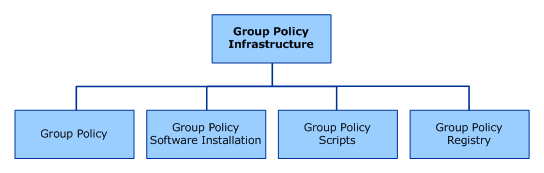
\includegraphics[width=0.75\columnwidth]{media/p05/jerarquiaEntidadesGp.png}
    \caption{Jerarquía de entidades administradas por la infraestructura de \textit{Group Policy}: el motor de directivas y las extensiones de cliente que leen los ajustes en los equipos destino \parencite{microsoftGroupPolicyInfra}.}
    \label{fig:jerarquiaEntidadesGp}
\end{figure}

La infraestructura de Group Policy se define como el mecanismo que entrega y aplica una o varias configuraciones deseadas a un conjunto de usuarios y computadoras destino dentro de un entorno de Active Directory, y se compone de un motor de directivas y de múltiples extensiones de cliente que se encargan de leer los ajustes concretos en los equipos destino \parencite{microsoftGroupPolicyInfra}. La Figura~\ref{fig:jerarquiaEntidadesGp} muestra su composición, con la extensión de registro, la de scripts y la de instalación de software como predecesoras de la aplicación directa de un objeto de política. Su propósito declarado es ofrecer una infraestructura de configuración centralizada del sistema operativo y de las aplicaciones que se ejecutan en él \parencite{microsoftGroupPolicy}. La Tabla~\ref{tab:objetosDirectorio} recoge los objetos que el despliegue deja creados en el directorio.

\begin{table}[H]
\centering
\small
\renewcommand{\arraystretch}{1.15}
\renewcommand{\tabularxcolumn}[1]{m{#1}}
\setlength{\emergencystretch}{1.5em}
\caption{Objetos creados en el directorio y función de cada uno en el despliegue.}
\label{tab:objetosDirectorio}
\begin{tabularx}{\textwidth}{>{\centering\arraybackslash}m{4.2cm} X}
\toprule
\textbf{Objeto del directorio} & \textbf{Función en el despliegue} \\
\midrule
\textbf{Unidad organizativa \textit{Clientes}} & Aloja las cuentas de los equipos que acceden al servidor, en particular el usuario \textit{clientewin}. \\
\addlinespace
\textbf{Unidad organizativa \textit{Servidores}} & Aloja las cuentas de servicio del propio servidor y de sus equipos administrativos. \\
\addlinespace
\textbf{Usuario clientewin} & Cuenta de la que valida el cliente nativo para las sesiones sobre el recurso compartido \textit{SoftwareRed}. \\
\addlinespace
\textbf{Grupo de dominio \textit{Administradores-SoftwareRed}} & Principal de seguridad al que se delegan los permisos sobre la carpeta compartida y que puede recibir directivas propias. \\
\addlinespace
\textbf{Objeto de política de grupo} & Conjunto de ajustes de configuración vinculados a una unidad organizativa para aplicarse a sus cuentas y equipos. \\
\bottomrule
\end{tabularx}
\end{table}

Conviene distinguir dos entidades de la configuración del ejercicio con nombres próximos. El grupo de trabajo Sistemas es una etiqueta de paridad entre equipos: no constituye un principal de seguridad, no admite la delegación de autoridad ni la aplicación de políticas, y únicamente permite que dos equipos intercambien recursos mediante la resolución de nombres NetBIOS. Un grupo de dominio, en cambio, es un objeto del directorio con identidad propia, al que se pueden conceder permisos sobre archivos y compartir y al que se puede vincular un objeto de política de grupo \parencite{microsoftADDSOverview}. La consecuencia práctica es que la cuenta clientewin se crea en el directorio del servidor y, mientras el cliente permanezca en el grupo de trabajo, sus sesiones se autentican de forma explícita contra esa cuenta en lugar de resolverse por la pertenencia a un dominio.

La contraseña de la cuenta clientewin se establece en el momento de su creación y no se consigna en esta documentación, por la misma razón que la guía de promoción desaconseja tratar las credenciales en claro \parencite{microsoftInstallADDS}: en un entorno real, una contraseña transcrita a un documento deja de ser un secreto.

\section{Servicio DNS}
\label{sec:servicioDns}

\subsection{Estructura del servicio, zonas y tipos de registros}
\label{sec:estructuraDns}

DNS es el protocolo industrial que asocia nombres de computadora con direcciones IP y hace posible la resolución de nombres para equipos y usuarios; en las redes de Windows es el servicio de resolución de nombres por omisión y forma parte de la capa de aplicación del modelo de referencia TCP/IP \parencite{microsoftDnsOverview}. El servicio cliente DNS viene incluido en todas las ediciones de Windows, se ejecuta por omisión tras la instalación y, en cuanto se configura una conexión TCP/IP con la dirección de un servidor DNS, realiza dos tareas: descubrir los controladores de dominio y resolver nombres de computadora en direcciones IP \parencite{microsoftDnsOverview}. La razón de ser del servicio está en la naturaleza del direccionamiento: los procesos remotos se identifican mediante la pareja nombre de host e identificador, y el nombre de host es alfanumérico en lugar de numérico porque resulta más fácil de recordar para las personas, aunque las computadoras prefieren los números por motivos de velocidad y simplicidad \parencite[\S 16.5.1, p.\ 567]{silberschatz2006fundamentos}.

DNS especifica tanto la estructura de nombrado de los hosts como la resolución de los nombres en direcciones, y el direccionamiento lógico se realiza con un nombre compuesto por múltiples partes, estructurado desde la más específica hasta la más general y con los campos separados por puntos \parencite[\S 16.5.1, p.\ 568]{silberschatz2006fundamentos}. El sistema resuelve las direcciones examinando los componentes del nombre en orden inverso: cada componente tiene un servidor de nombres ---un proceso en un sistema--- que acepta un nombre y devuelve la dirección del servidor responsable de ese nombre \parencite[\S 16.5.1, p.\ 568]{silberschatz2006fundamentos}. Para \textit{bob.cs.brown.edu}, el núcleo del sistema solicitante pide al servidor de nombres del dominio \textit{edu} la dirección del de \textit{brown.edu}; con ella consulta a este último por \textit{cs.brown.edu} y solicita el identificador de bob.cs.brown.edu, que responde con un identificador en forma de dirección Internet \parencite[\S 16.5.1, p.\ 568]{silberschatz2006fundamentos}. El protocolo puede parecer poco eficiente, pero cada servidor de nombres mantiene cachés locales que aceleran el proceso y deben refrescarse por si un servidor se traslada; frente a la caída del servidor principal de un dominio, la solución consiste en servidores de nombres secundarios de reserva que dupliquen su contenido \parencite[\S 16.5.1, p.\ 569]{silberschatz2006fundamentos}.

Cada entrada de la base de datos de nombres es un registro de recurso con un formato fijo: un nombre de propietario, un tipo, una clase, un tiempo de vida, la longitud y los datos \parencite[\S 3.2.1, p.\ 11]{rfc1035}. El tiempo de vida es un entero de 32 bits que especifica el intervalo durante el cual el registro puede quedar almacenado en caché antes de volver a consultar a la fuente de la información; un valor cero significa que el registro solo puede usarse en la transacción en curso y no debe almacenarse, y por esa razón los registros de inicio de autoridad se distribuyen siempre con tiempo de vida cero para impedir su almacenamiento en caché \parencite[\S 3.2.1, p.\ 11]{rfc1035}. La Tabla~\ref{tab:tiposRegistroDns} recoge los tipos que el despliegue utiliza o que el mecanismo de directorio exige.

\begin{table}[H]
\centering
\small
\renewcommand{\arraystretch}{1.15}
\renewcommand{\tabularxcolumn}[1]{m{#1}}
\setlength{\emergencystretch}{1.5em}
\caption{Tipos de registro de recurso empleados en el despliegue y función de cada uno.}
\label{tab:tiposRegistroDns}
\begin{tabularx}{\textwidth}{>{\centering\arraybackslash}m{2.4cm} X X}
\toprule
\textbf{Tipo} & \textbf{Significado} & \textbf{Uso en el despliegue} \\
\midrule
\textbf{A} & Dirección de un host. & Registro del nombre del servidor con su dirección IPv4 en la zona del dominio, acompañado del tipo AAAA, que almacena una sola dirección IPv6 de 128 bits en orden de bytes de red y lleva el valor de tipo 28 que le asignó la IANA \parencite[\S 2.1, p.\ 3]{rfc3596}. \\
\addlinespace
\textbf{NS} & Servidor de nombres autoritativo. & Publica qué servidores son autoritativos para cada zona. \\
\addlinespace
\textbf{CNAME} & Nombre canónico de un alias. & Permite que un nombre alternativo apunte al nombre verdadero. \\
\addlinespace
\textbf{PTR} & Puntero a un nombre de dominio. & Registro inverso que asocia una dirección a su nombre, en la zona inversa. \\
\addlinespace
\textbf{SOA} & Marca el inicio de una zona de autoridad. & Define el servidor principal de la zona y los parámetros de replicación y de caducidad. \\
\addlinespace
\textbf{SRV} & Localización de servicios (Service Record); permite varios servidores para un mismo dominio, trasladar servicios de un host a otro con pocas complicaciones y designar hosts primarios y de reserva para un servicio \parencite[\S 1, p.\ 1]{rfc2782}. & Registra los puntos de contacto de los servicios de directorio y de aplicación, con el formato \texttt{\_Service.\_Proto.Name TTL Class SRV Priority Weight Port Target}. \\
\bottomrule
\end{tabularx}
\end{table}

El espacio de nombres puede dividirse en una o más zonas, que se almacenan, distribuyen y replican a otros servidores DNS, y la partición responde a tres motivos: delegar la gestión de una parte del espacio de nombres en otra ubicación, dividir una zona grande en zonas menores para distribuir la carga de tráfico entre varios servidores y mejorar el rendimiento o la tolerancia a fallos, y extender el espacio de nombres añadiendo numerosos subdominios de una sola vez \parencite{microsoftZoneDelegation}. Cuando se crea una zona primaria estándar, toda la información de registros de recurso se almacena en un archivo de texto en un único servidor DNS que actúa como maestro principal de la zona, y la información se replica a los demás \parencite{microsoftZoneDelegation}. Al delegar una zona hija, la zona matriz debe incluir los registros que la hacen autoritativa: uno de servidor de nombres que advertise la delegación y otro de host que resuelve el nombre del servidor delegado, conocido como registro de enlace \parencite{microsoftZoneDelegation}. La Figura~\ref{fig:delegacionZonaDns} muestra ese mecanismo.

\begin{figure}[htbp]
    \centering
    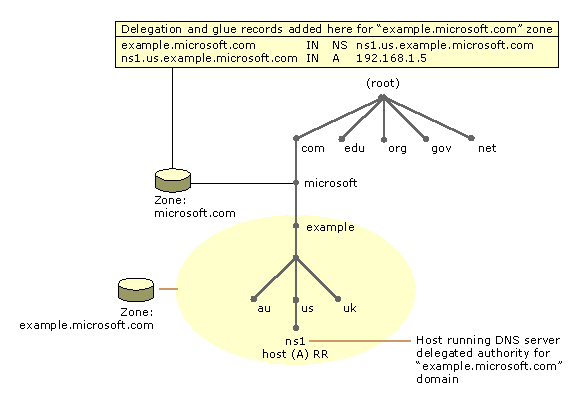
\includegraphics[width=0.72\columnwidth]{media/p05/delegacionZonaDns.png}
    \caption{Delegación de una zona hija dentro de la zona matriz, con los registros de servidor de nombres y de enlace que la zona matriz debe escribir \parencite{microsoftZoneDelegation}}.
    \label{fig:delegacionZonaDns}
\end{figure}

\subsection{Integración con AD DS y resolución de nombres del servidor}
\label{sec:integracionDnsAd}

El servicio DNS no es un componente accesorio del directorio: es el mecanismo mediante el cual AD DS localiza a los controladores de dominio para las operaciones de autenticación, actualización y búsqueda, y los propios controladores de dominio lo emplean para localizarse entre sí \parencite{microsoftDnsOverview}. El servidor DNS es además el responsable de almacenar y replicar las zonas que contienen los nombres y las direcciones IP de todas las computadoras del dominio \parencite{microsoftDnsOverview}. Por esa razón la instalación de un bosque nuevo incorpora el servicio DNS de manera automática \parencite{microsoftDnsOverview}, y el propio rol lo define como el que proporciona el método estándar para asociar nombres con direcciones numéricas de Internet, de modo que los usuarios puedan referirse a las computadoras mediante nombres fáciles de recordar \parencite{microsoftRoleDNSServer}.

La promoción descrita en la sección anterior dejó por tanto el servidor con dos artefactos que gobiernan el capítulo de nombres: la zona primaria sistemas.lab, autoritativa sobre el dominio, y los registros que el propio controlador de dominio publica en ella ---su registro de host, los registros de servidor de nombres que lo designan autoritativo y los registros SRV que localizan los servicios de directorio---. El mantenimiento de esos registros se apoya en la actualización dinámica, que permite el registro y la actualización automática de los registros de los clientes \parencite{microsoftDnsOverview}. El servicio se administra con su consola de administración, en la que la pestaña de reenviadores permite indicar las direcciones de los servidores DNS a los que se delegan las consultas que el servidor no puede resolver localmente \parencite{microsoftDnsQuickstart}.

La resolución de nombres del propio servidor debe cerrarse sobre sí mismo para no depender del anfitrión: al quedar la máquina virtual en modo puente, su dirección pertenece a la red física y el equipo anfitrión puede tener un servidor DNS propio ---o ninguno--- que no resuelva los nombres del dominio recién creado. La Tabla~\ref{tab:configuracionDns} recoge la configuración de nombres que se aplica al servidor y al cliente nativo.

\begin{table}[H]
\centering
\small
\renewcommand{\arraystretch}{1.15}
\renewcommand{\tabularxcolumn}[1]{m{#1}}
\setlength{\emergencystretch}{1.5em}
\caption{Configuración de resolución de nombres del servidor y del cliente nativo.}
\label{tab:configuracionDns}
\begin{tabularx}{\textwidth}{>{\centering\arraybackslash}m{4.2cm} X}
\toprule
\textbf{Elemento} & \textbf{Valor y fundamento} \\
\midrule
\textbf{Servidor DNS preferido del servidor} & La propia dirección IP del servidor. La resolución de los nombres del dominio no debe depender de un servicio ajeno a la red del ejercicio, y el bucle se resuelve porque la zona es autoritativa y local. \\
\addlinespace
\textbf{Sufijo DNS del servidor} & sistemas.lab, que hace que las consultas sin sufijo se resuelvan dentro del dominio. \\
\addlinespace
\textbf{Forwarders del servidor} & Ninguno. En una red aislada no existe un orden superior al que remitir, y remitir las consultas dejaría sin resolver las que no pertenecen al dominio. \\
\addlinespace
\textbf{Servidor DNS preferido del cliente} & La dirección IP del servidor. Es el único servicio de nombres que el cliente nativo puede consultar para alcanzar los recursos del dominio. \\
\addlinespace
\textbf{Nombre de NetBIOS del cliente} & Registrado en el servicio, de modo que el servidor también lo resuelve por su nombre de equipo. \\
\bottomrule
\end{tabularx}
\end{table}

La verificación del servicio se realiza con las utilidades de línea de comandos del propio sistema operativo: la resolución se comprueba consultando al servidor y la configuración de la conexión se contrasta con el resultado de \textit{ipconfig}, que muestra el servidor DNS preferido y el sufijo DNS activo \parencite{microsoftDnsOverview}. Los reenviadores vacíos no impiden resolver los nombres del dominio, pero sí cualquier nombre externo, de modo que el cliente nativo no alcanzará recursos de Internet por nombre mientras no se añada un reenviador; para el alcance local del ejercicio esa limitación es aceptable y reduce además la superficie de exposición del servidor.

\section{Servicios de archivos y almacenamiento}
\label{sec:serviciosArchivos}

\subsection{Rol File Services: recursos compartidos, cuotas y DFS}
\label{sec:rolFileServices}

El rol File Services agrupa las tecnologías que administran el almacenamiento, permiten la replicación de archivos, gestionan las carpetas compartidas, apresuran la búsqueda de archivos y habilitan el acceso de computadoras UNIX \parencite{microsoftRoleFileServices}. En la versión instalada ese conjunto comprende los recursos compartidos, los espacios de nombres y la replicación del sistema de archivos distribuido (DFS), el Administrador de recursos de servidor de archivos con sus cuotas, los archivos y carpetas sin conexión, los servicios para NFS y la caché de sucursales \parencite{microsoftFileServices2008r2}. El servicio se apoya en el protocolo Server Message Block (SMB) como subyacente: el servidor SMB comparte recursos ---archivos, impresoras y conductos con nombre--- y atiende las peticiones de los clientes, mientras que el cliente SMB se conecta a los recursos remotos, de manera que el acceso a una ruta UNC (Universal Naming Convention) es iniciado y gestionado por el cliente \parencite{microsoftSmbOverview}. SMB es además el protocolo de base de los servicios de archivos de Windows Server, entre ellos los espacios de nombres DFS, que organizan carpetas compartidas de varios servidores en un espacio de nombres lógico \parencite{microsoftSmbOverview}.

El acceso a los recursos compartidos se realiza sobre el puerto TCP 445, y el análisis de buenas prácticas del servicio de archivos señala que, si los puertos necesarios para compartir archivos e impresoras no están abiertos en el cortafuegos, los equipos no pueden acceder a las carpetas compartidas \parencite{microsoftSmbPorts}; la apertura del puerto corresponde a las reglas que el rol incorpora al instalarse sobre el cortafuegos que el despliegue deja activo \parencite{microsoftInstallWs2008r2}.

\subsection{Carpeta compartida SoftwareRed: permisos de uso frente a NTFS}
\label{sec:carpetaSoftwareRed}

La carpeta que el ejercicio exige compartir se crea en el volumen del sistema con el nombre SoftwareRed y se comparte bajo ese mismo nombre, de modo que el cliente la alcanza con la ruta \texttt{\textbackslash\textbackslash SRV-SISTEMAS\textbackslash SoftwareRed}. El punto que decide el funcionamiento del recurso es que el acceso se autoriza en dos capas independientes y ambas deben permitir la operación: los permisos del recurso compartido, que se editan en la pestaña Compartir mediante Compartir avanzado, y los permisos NTFS de la carpeta física, que se editan en la pestaña Seguridad \parencite{microsoftShareNtfsPermissions}. La publicación exige retirar el grupo \textit{Todos} de los permisos del recurso y añadir el usuario o grupo concreto que debe acceder, con los permisos de Control total, Cambiar o Leer; el procedimiento paralelo sobre la estructura de carpetas añade los usuarios o grupos en cada nivel y especifica los permisos de Control total, Modificar, Leer y ejecutar, Enumerar contenido de carpeta, Leer, Escribir y permisos especiales \parencite{microsoftShareNtfsPermissions}. La propia documentación de diagnóstico confirma la exigencia de las dos capas al presentar como solución al error de falta de permisos tanto la concesión del permiso en el recurso compartido como la del permiso NTFS correspondiente \parencite{microsoftSharedFolderAccess}.

El modelo de derechos de acceso que se aplica a la carpeta tiene una estructura jerárquica bien definida: el propietario del archivo posee todos los derechos y puede otorgarlos a otros, y cada derecho implica los que le preceden, de modo que quien tiene el derecho de actualización posee también el de conocimiento, ejecución, lectura y anexión \parencite[\S 12.5, p.\ 569]{stallings2018operating}. El acceso puede concederse a un usuario concreto, a un grupo de usuarios o a todos los que tienen acceso al sistema, y esa misma clasificación es la que se reproduce en la configuración de la carpeta compartida \parencite[\S 12.5, p.\ 570]{stallings2018operating}. La Tabla~\ref{tab:permisosSoftwareRed} recoge la asignación por principal.

\begin{table}[H]
\centering
\small
\renewcommand{\arraystretch}{1.15}
\renewcommand{\tabularxcolumn}[1]{m{#1}}
\setlength{\emergencystretch}{1.5em}
\caption{Permisos concedidos sobre la carpeta compartida SoftwareRed por principal.}
\label{tab:permisosSoftwareRed}
\begin{tabularx}{\textwidth}{>{\centering\arraybackslash}m{3.8cm} m{3.0cm} X}
\toprule
\textbf{Principal} & \textbf{Permiso de recurso} & \textbf{Permiso NTFS en la carpeta física} \\
\midrule
\textbf{Administradores} & Control total. & Control total. \\
\addlinespace
\textbf{Sistema} & --- & Control total. \\
\addlinespace
\textbf{clientewin} & Cambiar. & Modificar. \\
\addlinespace
\textbf{Grupo de dominio Administradores-SoftwareRed} & Cambiar. & Modificar. \\
\addlinespace
\textbf{Todos} & Retirado. & Sin entradas. \\
\bottomrule
\end{tabularx}
\end{table}

El reparto entre las dos capas no es redundante: los permisos del recurso compartido constituyen el filtro de entrada al recurso, mientras que los permisos NTFS siguen protegiendo la carpeta cuando esta se alcanza por otra vía ---por ejemplo de forma local o a través de una copia---, y el acceso efectivo de una sesión es la intersección de lo que ambas capas conceden \parencite{microsoftShareNtfsPermissions}. Los comandos equivalentes en línea de órdenes, que producen exactamente la misma configuración y que permiten verificar su estado, son los siguientes.

\begin{mdframed}[style=terminal]
\ttfamily\upshape\color{bashLetterColor}\footnotesize
net share SoftwareRed=C\textbackslash SoftwareRed /grant:clientewin:Change \textbackslash\\
\ \ /grant:Administradores-SoftwareRed:Change \textbackslash\\
\ \ /grant:Administradores:FULL
icacls C\textbackslash SoftwareRed /grant clientewin:(OI)(CI)M \textbackslash\\
\ \ /grant Administradores-SoftwareRed:(OI)(CI)M \textbackslash\\
\ \ /remove Everyone
\end{mdframed}

\subsection{Administración de archivos compartidos y MMC}
\label{sec:administracionArchivos}

La administración del rol se realiza desde la consola de administración de archivos y almacenamiento y desde el nodo de File Services de Server Manager, que permiten crear y modificar los recursos compartidos, configurar las cuotas de disco y definir los espacios de nombres DFS \parencite{microsoftFileServices2008r2}. El propio rol incorpora un analizador de buenas prácticas específico que examina la configuración del servidor de archivos y detecta, entre otras incidencias, los puertos de compartición de archivos e impresoras cerrados en el cortafuegos \parencite{microsoftSmbPorts} \parencite{microsoftFileServices2008r2}.

La verificación desde el lado del cliente tiene una taxonomía de errores que permite localizar la causa sin ambigüedad. La ruta de red no encontrada ---error de sistema 53--- se produce cuando el servidor no llega a recibir la solicitud de conexión; la causa habitual es que el servicio auxiliar NetBIOS sobre TCP/IP esté detenido o se ejecute con una identidad de cuenta inadecuada, y la comprobación de conectividad con el puerto 445 mediante \textit{telnet} permite distinguir el problema de red del de resolución de nombres \parencite{microsoftSharedFolderAccess}. El error de falta de permiso sobre la ruta indica que la cuenta autenticada no tiene concedido el acceso en ninguna de las dos capas \parencite{microsoftSharedFolderAccess}. Y el bloqueo del acceso invitado no autenticado por las políticas de seguridad de la organización, que es el escenario con el que se topa un cliente que permanece en el grupo de trabajo, se resuelve habilitando los inicios de sesión invitados no seguros mediante una directiva de configuración \parencite{microsoftSharedFolderAccess}.

\section{Servidor de aplicaciones e IIS 7.5}
\label{sec:servidorAplicacionesIis}

\subsection{Rol Application Server: COM+, MS DTC, WCF}
\label{sec:rolApplicationServer}

El rol Application Server constituye un entorno integrado para desplegar y ejecutar aplicaciones de negocio propias, basadas en servidor, que atienden peticiones que llegan por la red desde equipos clientes remotos o desde otras aplicaciones \parencite{microsoftApplicationServerRole} \parencite{microsoftRoleApplicationServer}. Sus servicios de rol se apoyan en tres tecnologías de la plataforma Windows: el modelo de objetos de componentes (COM+), el coordinador de transacciones distribuidas de Microsoft (MS DTC) y Windows Communication Foundation (WCF). El rol admite aplicaciones construidas con el .NET Framework 3.0 y da soporte a las que emplean COM+, Message Queuing, servicios web y transacciones distribuidas \parencite{microsoftRoleApplicationServer}. Su criterio de uso es explícito: se recomienda cuando las aplicaciones que se van a desplegar dependen de alguna de las tecnologías que el rol integra ---IIS, .NET Framework, ASP.NET, COM+, Message Queuing o servicios web construidos con Windows Communication Foundation--- y cuando el desarrollador ha indicado qué servicios de rol son necesarios; no todos los servidores de aplicaciones se benefician de él, pues el rol no es necesario para sostener Microsoft Exchange Server ni Microsoft SQL Server \parencite{microsoftApplicationServerRole}.

Lo que el rol aporta se reduce a tres cosas: un entorno de ejecución que permite desplegar y administrar aplicaciones de negocio de alto rendimiento que atienden peticiones desde navegadores de la red pública o de la intranet y desde sistemas remotos que envían peticiones como mensajes; el .NET Framework 3.0, que aporta un modelo de programación simplificado para aplicaciones conectadas y, para el administrador, un entorno de ejecución seguro y de alto rendimiento junto con un entorno simplificado de configuración y despliegue; y el asistente de instalación de roles, que instala automáticamente todas las características necesarias para cada servicio de rol seleccionado \parencite{microsoftApplicationServerRole}. Sobre la línea base del .NET Framework 2.0, que ya incluye el Common Language Runtime (CLR) con su entorno de ejecución seguro y su soporte de interoperabilidad entre lenguajes, el rol instala Application Server Foundation, que es esencialmente el .NET Framework 3.0 y aporta como componentes clave WCF, Windows Workflow Foundation y Windows Presentation Foundation \parencite{microsoftApplicationServerRole}.

WCF es el modelo de programación unificado de Microsoft para construir aplicaciones conectadas que se comunican mediante servicios web ---las llamadas aplicaciones orientadas a servicio---, y permite componer de manera coherente las tecnologías preexistentes para aplicaciones distribuidas: COM+ y los servicios de empresa de .NET, Message Queuing, .NET Remoting, los servicios web de ASP.NET y Web Services Enhancements \parencite{microsoftApplicationServerRole}. Los servicios de rol del cuadro siguiente expresan el alcance real del rol en el despliegue.

\begin{table}[H]
\centering
\small
\renewcommand{\arraystretch}{1.15}
\renewcommand{\tabularxcolumn}[1]{m{#1}}
\setlength{\emergencystretch}{1.5em}
\caption{Servicios de rol de Application Server y su función.}
\label{tab:serviciosRolApplicationServer}
\begin{tabularx}{\textwidth}{>{\centering\arraybackslash}m{4.4cm} X}
\toprule
\textbf{Servicio de rol} & \textbf{Función} \\
\midrule
\textbf{Web Server} & Instala el servidor web Internet Information Services (IIS) y permite alojar sitios o servicios internos o externos con contenido estático o dinámico, aplicaciones ASP.NET y servicios web construidos con WCF o ASP.NET. \\
\addlinespace
\textbf{Acceso a red de COM+} & Permite la invocación remota de aplicaciones construidas sobre componentes COM+ y de Servicios de empresa. \\
\addlinespace
\textbf{Servicio de activación de procesos de Windows} & Inicia y detiene aplicaciones dinámicamente según los mensajes recibidos por HTTP, Message Queuing, TCP y conductos con nombre, de modo que los recursos del servidor se emplean con mayor eficiencia. \\
\addlinespace
\textbf{Compartir puertos de Net.TCP} & Permite que varias aplicaciones empleen un mismo puerto TCP mediante multiplexión, extremo que se hace necesario cuando las reglas del cortafuegos sólo dejan abiertos unos pocos puertos. \\
\addlinespace
\textbf{Transacciones distribuidas} & Proporciona semántica de todo o nada para las actualizaciones que se realizan sobre varias bases de datos u otros recursos transaccionales. \\
\bottomrule
\end{tabularx}
\end{table}

El rol Application Server no está disponible en la edición Windows Web Server 2008 y sí en las ediciones Standard, Enterprise, Datacenter y para sistemas Itanium \parencite{microsoftApplicationServerRole}; esta exclusión es una de las razones que justifican la elección de la edición Standard realizada en el capítulo de instalación.

\subsection{IIS 7.5: arquitectura modular, application pools y módulos}
\label{sec:iis75Arquitectura}

IIS 7.5 es el rol Web Server (IIS) de Windows Server 2008 R2, mientras que IIS 7.0 corresponde a Windows Server 2008 \parencite{microsoftUnderstandingIisSetup}; la versión de IIS constituye el servidor web de Windows Server 7 \parencite{microsoftRoleWebServerIIS}. El servidor web fue rediseñado en IIS 7.0 para permitir la personalización del equipo mediante la adición o la eliminación de módulos, y un módulo es una característica individual que el servidor emplea para procesar las peticiones: las versiones 7.0 y 7.5 emplean módulos de autenticación para validar las credenciales del cliente y módulos de caché para administrar la actividad de caché \parencite{microsoftInstallIis7}.

El diseño de instalación de IIS 7 y superiores es completamente modular, lo que permite controlar la huella del servidor web, y la arquitectura de canalización aporta un alto grado de granularidad: más de cuarenta características seleccionables que permiten desplegar servidores muy delgados y específicos para una tarea y bloquear funcionalidad que antes no era posible \parencite{microsoftUnderstandingIisSetup}. El cambio de fondo respecto de IIS 6.0 es arquitectónico: en la versión anterior las características no deseadas se instalaban y quedaban desactivadas, pero seguían consumiendo CPU y memoria y exigían parches, mientras que en IIS 7 no se instalan siquiera \parencite{microsoftUnderstandingIisSetup}. La instalación se apoya en la misma tecnología por componentes que el sistema operativo, con un modelo declarativo que aporta una base de binarios única, dependencias conocidas para cada característica que permiten paquetes de servicio más pequeños y una superficie de ataque reducida \parencite{microsoftUnderstandingIisSetup}.

La Figura~\ref{fig:arquitecturaIis75} resume la organización del servicio en el nivel de componentes instalados y en el de proceso de atención de peticiones.

\begin{figure}[htbp]
\centering
\begin{minipage}{0.95\textwidth}
\begin{localsubgroup}
IIS 7.5
\begin{localsubgroup}
- Características del rol web \\
- Servicio de activación de procesos \\
\begin{localsubgroup}
- Modelo de procesos \\
- Grupo de aplicaciones
\end{localsubgroup}
- Módulos de la canalización
\end{localsubgroup}
\end{localsubgroup}
\end{minipage}
\caption{Organización de IIS 7.5: características instaladas, servicio de activación de procesos y grupo de aplicaciones con su proceso de trabajo \parencite{microsoftUnderstandingIisSetup}.}
\label{fig:arquitecturaIis75}
\end{figure}

El servicio de activación de procesos de Windows aporta la infraestructura de activación y de gestión de procesos y también la de procesamiento HTTP, y todas las características del grupo de actualización IIS-WebServer dependen de él \parencite{microsoftUnderstandingIisSetup}. Esa dependencia no es un detalle del asistente: al seleccionar el rol Web Server, el asistente de instalación de roles la detecta y ofrece añadir los servicios de rol requeridos \parencite{microsoftInstallIis7}. El mecanismo de activación se apoya en el modelo de procesos, que es el que materializa el aislamiento mediante los grupos de aplicaciones: cada aplicación web se atiende en un proceso de trabajo propio, de manera que el fallo de una no afecta a las demás y cada grupo puede tener su propia identidad de seguridad. Ese aislamiento por proceso sustituye al modelo monolítico de IIS 6.0, donde todas las aplicaciones compartían un único espacio de proceso.

La configuración dejó atrás la metabase de IIS 6.0: la instalación por omisión de IIS 7.5 aporta un servidor de contenido estático con administración local y autenticación anónima ---esta última siempre presente con cualquier característica de servidor web--- y, por cada componente instalado, su configuración predeterminada se añade al almacén unificado \textit{ApplicationHost.config} \parencite{microsoftUnderstandingIisSetup}. Ese almacén, editable en un archivo de texto plano, es la razón de que la nueva interfaz de administración cambie con rapidez los ajustes de cada sitio y delegue en los propietarios de sitios el control administrativo \parencite{microsoftInstallIis7}. IIS 7.5 añade además a su predecesor el registro y el rastreo de los cambios de configuración, de los que IIS 7.0 carece, y el analizador de buenas prácticas \parencite{microsoftInstallIis7}.

\subsection{Publicación del sitio, enlace de puerto y prueba HTTP}
\label{sec:publicacionSitio}

La incorporación del rol se realiza desde Server Manager: en Roles Summary se inicia el asistente de instalación de roles, se selecciona Web Server (IIS) en la página de selección de roles de servidor y, en la página de servicios de rol, se marcó el conjunto mínimo necesario en lugar de aceptar la instalación por omisión, que incluye un conjunto mínimo de servicios de rol \parencite{microsoftInstallIis7}. La propia documentación es explícita en la recomendación: instalar solo los servicios de IIS absolutamente necesarios para minimizar la huella de la instalación y con ella la superficie de ataque \parencite{microsoftInstallIis7}.

La publicación de un sitio consta de cuatro objetos enlazados entre sí. El primero es la ruta física, que es el directorio del disco donde reside el contenido y que se crea con el sistema de archivos NTFS descrito en el capítulo de arquitectura interna. El segundo es el sitio, que es el espacio de nombres lógico al que se asocian uno o más enlaces, entendidos como las combinaciones de protocolo, nombre de host y puerto que dirigen el tráfico entrante a un sitio concreto. El tercero es el grupo de aplicaciones, que es el contenedor que aporta el aislamiento mediante el proceso de trabajo y que define la identidad de seguridad con la que se ejecutan las peticiones. El cuarto es el documento predeterminado, que es el archivo que se sirve cuando la dirección solicitada no especifica ninguno.

\begin{mdframed}[style=terminal]
\ttfamily\upshape\color{bashLetterColor}\footnotesize
appcmd add site "Intranet" "C:\textbackslash inetpub\textbackslash Intranet" \textbackslash\\
appcmd set site "Intranet" /bindings:*:80:SRV-SISTEMAS \textbackslash\\
appcmd add apppool "Intranet" /managedRuntimeVersion:v4.0 \textbackslash\\
appcmd set app "Intranet/" /applicationPool:"Intranet" \textbackslash\\
appcmd set config "Intranet" /section:system.webServer/ \textbackslash\\
\ \ /[entry\#"defaultDocument"]/@value:"index.htm"
\end{mdframed}

El enlace de puerto es la decisión que hace visible el servicio desde el cliente nativo: con el enlace en el puerto 80 y el nombre de host del servidor, la dirección \texttt{http://SRV-SISTEMAS/} queda disponible para cualquier equipo de la LAN, y la regla de entrada del cortafuegos que el rol incorpora permite el tráfico entrante hacia ese puerto. La verificación se realiza en dos niveles: en el propio servidor, consultando la dirección local \texttt{http://localhost}, que debe devolver la página de bienvenida, y desde el cliente nativo, que abre la misma ruta en su navegador. Cada petición atendida queda registrada por el módulo de registro HTTP ---habilitado en la instalación por omisión--- en el archivo del servicio W3SVC, lo que permite confirmar que la petición llegó realmente al servicio y no se quedó en una etapa anterior de la resolución de nombres o del cortafuegos.

\section{Cliente nativo e integración}
\label{sec:clienteNativo}

\subsection{Configuración del cliente en el grupo de trabajo Sistemas}
\label{sec:configuracionCliente}

El cliente es la computadora nativa del ejercicio y no la máquina virtual, y esa condición determina el modo en que se autentican sus sesiones. La máquina permanece en el grupo de trabajo Sistemas, que es una etiqueta de paridad entre equipos y no un dominio: no existe un Ticket de servicio que emita, no hay Kerberos ni resolución de nombres de dominio, y el acceso a los recursos del servidor exige presentar credenciales de forma explícita \parencite{microsoftADDSOverview}. La pertenencia al grupo aporta sin embargo una ventaja concreta: la resolución de nombres NetBIOS, que permite que ambos equipos se localicen mutuamente por su nombre de equipo.

La configuración del cliente comprende cuatro acciones. La primera es la incorporación al grupo de trabajo, desde las propiedades del sistema, en la pestaña del nombre de equipo, que es el mecanismo homólogo al que el servidor emplea en sus tareas de configuración inicial para incorporarse a un dominio \parencite{microsoftInstallWinServer2008}. La segunda es la dirección del servidor DNS preferido, que debe apuntar a la del servidor, de modo que el servicio cliente DNS ---presente en todas las ediciones de Windows y ejecutado por omisión--- resuelva tanto los nombres de computadora como el descubrimiento de controladores de dominio \parencite{microsoftDnsOverview}. La tercera es la habilitación del acceso a archivos e impresoras en la configuración avanzada de compartición, donde se activan la detección de red y la compartición de archivos e impresoras, sin lo cual el equipo no es visible en la red \parencite{microsoftSharedFolderAccess}. La cuarta es el permiso del cortafuegos del cliente para el tráfico de entrada de la compartición de archivos \parencite{microsoftSmbPorts}.

\subsection{Cuenta clientewin y montaje del recurso compartido}
\label{sec:cuentaClienteWin}

La cuenta clientewin se creó en el capítulo del directorio activo como objeto de usuario dentro de la unidad organizativa Clientes, con la contraseña fijada en el momento de su creación, y es a ella a quien se concedieron los permisos de recurso compartido y NTFS sobre la carpeta SoftwareRed. Al conservar el cliente en el grupo de trabajo, esa cuenta no se resuelve de forma transparente: el sistema operativo del cliente debe indicarla de forma explícita y completa, con el nombre del dominio como prefijo, porque de lo contrario intentaría resolverla en el contexto del grupo de trabajo y no la encontraría.

\begin{mdframed}[style=terminal]
\ttfamily\upshape\color{bashLetterColor}\footnotesize
net use \textbackslash\textbackslash SRV-SISTEMAS\textbackslash SoftwareRed \textbackslash\\
\ \ /user:SISTEMAS.LAB\textbackslash clientewin *
net use
dir \textbackslash\textbackslash SRV-SISTEMAS\textbackslash SoftwareRed
\end{mdframed}

El asterisco al final de la línea de órdenes no es un comodín de directorio, sino la indicación de que el sistema debe solicitar la contraseña de forma interactiva en lugar de leerla de la línea de órdenes, que es el comportamiento que evita dejar la credencial en el historial de la consola \parencite{microsoftSharedFolderAccess}. La orden \textit{net use} sin argumentos enumera las conexiones activas, y el listado del recurso mediante una ruta UNC comprueba que el montaje se realizó y que los permisos concedidos en las dos capas son los suficientes. La ruta UNC es exactamente la que inicia y gestiona el cliente SMB del sistema operativo \parencite{microsoftSmbOverview}.

\subsection{Batería de verificación de los cuatro servicios}
\label{sec:verificacionServicios}

La comprobación final no puede limitarse a la apertura del recurso compartido, porque el ejercicio exige cuatro servicios y cada uno falla de una forma distinta. La Tabla~\ref{tab:bateriaVerificacion} fija, para cada servicio, la prueba que lo acredita y el resultado esperado, de modo que un fallo quede localizado sin ambigüedad.

\begin{table}[H]
\centering
\small
\renewcommand{\arraystretch}{1.15}
\renewcommand{\tabularxcolumn}[1]{m{#1}}
\setlength{\emergencystretch}{1.5em}
\caption{Batería de verificación de los cuatro servicios desde el cliente nativo.}
\label{tab:bateriaVerificacion}
\begin{tabularx}{\textwidth}{>{\centering\arraybackslash}m{3.2cm} m{5.0cm} X}
\toprule
\textbf{Servicio} & \textbf{Prueba} & \textbf{Resultado esperado} \\
\midrule
\textbf{DNS} & Consulta del nombre del servidor al servicio DNS configurado como preferido. & Devuelve la dirección IP del servidor, lo que confirma la resolución de nombres y descarta un problema de conectividad. \\
\addlinespace
\textbf{Directorio activo} & Enumeración de los recursos compartidos del servidor mediante su nombre NetBIOS. & Presenta el recurso SoftwareRed y el recurso administrativo \textit{IPC\$}, lo que acredita que el servidor atiende el protocolo de compartición como controlador de dominio. \\
\addlinespace
\textbf{Archivos} & Montaje del recurso con las credenciales explícitas de la cuenta y listado de su contenido. & La conexión se establece y el contenido de la carpeta aparece, lo que confirma los permisos de recurso compartido y NTFS sobre el directorio. \\
\addlinespace
\textbf{Servidor de aplicaciones} & Petición HTTP al nombre del servidor desde el navegador y consulta del registro del servicio. & El navegador muestra la página publicada y el registro W3SVC registra la petición, lo que demuestra que la petición alcanzó el proceso de trabajo y no se detuvo en el cortafuegos ni en la resolución de nombres. \\
\bottomrule
\end{tabularx}
\end{table}

El orden de las pruebas no es arbitrario y conviene respetarlo, porque cada una descarta un eslabón distinto. La resolución de nombres es la primera porque, sin ella, las tres restantes fallarían por un motivo ajeno al servicio que se pretende comprobar. La enumeración de recursos viene después porque exige que el servidor atienda el protocolo de compartición, lo que presupone que el servicio de archivos está activo y que el cortafuegos admite el tráfico entrante. La apertura de la carpeta prueba por último la cadena completa, porque combina la resolución de nombres, la autenticación con credenciales explícitas y la aplicación de los dos niveles de permisos. Y la prueba HTTP se realiza en último lugar porque es la única que no depende del grupo de trabajo: se sostiene sobre el nombre del host y el puerto del enlace, de modo que su fallo aísla el servicio de aplicaciones sin arrastrar el diagnóstico de los anteriores.

Un último matiz sobre el resultado de la enumeración: la presentación del recurso administrativo IPC\$ confirma que el servidor actúa como controlador de dominio, y ese recurso se encuentra oculto de la enumeración ordinaria, de manera que solo se alcanza indicando la ruta completa \parencite{microsoftShareNtfsPermissions}. Esa distinción es la que permite al administrador confirmar el papel del servidor sin exponerlo en la lista de recursos compartidos.

\section{Conclusiones}
\label{sec:conclusiones}

El despliegue de un servidor Windows Server 2008 R2 completo sobre una máquina virtual ha resultado más exigente de lo que sugiere la simple enumeración de los servicios solicitados, porque los cuatro roles que el enunciado enumera no son componentes independientes sino capas que se apoyan unas en otras y que, por tanto, solo funcionan si el orden de su incorporación es el correcto. La observación de mayor alcance que se desprende del trabajo es que el directorio activo no es un servicio más entre los demás, sino el sustrato sobre el que se apoyan el servicio de nombres y la autenticación de las sesiones; el servicio DNS, a su vez, no es un resolvedor de nombres commodities sino el mecanismo que permite localizar al controlador de dominio, y sin él la promoción del servidor a controlador de dominio no habría sido posible ni verificable. De la misma manera, el recurso compartido que el cliente consume sólo es alcanzable si existe una ruta de nombres desde la máquina nativa hasta el servidor, y esa ruta existe únicamente porque la red virtual está en modo puente y no en modo de traducción de direcciones, decisión de configuración que parece menor y que en realidad determina si el ejercicio tiene sentido.

El trabajo ha permitido también comprobar de forma práctica una afirmación que suele quedar en el terreno de la teoría: la diferencia entre un modelo de permisos de recurso compartido y un modelo de permisos del sistema de archivos no es un matiz administrativo, sino un mecanismo de defensa en profundidad. Un acceso denegado en un recurso compartido puede deberse a que ninguna de las dos capas concede el permiso, y el diagnóstico exige consultar ambas por separado, porque un permiso aparentemente correcto en la interfaz del recurso puede quedar anulado por una entrada de control de acceso más restrictiva en la carpeta física. Esa misma lógica de capas se repite, a otra escala, en la arquitectura del sistema operativo que sostiene el despliegue: el sistema de archivos NTFS protege la estructura de sus metadatos mediante un registro transaccional que garantiza la consistencia de las estructuras internas, aunque no la del contenido de los archivos de usuario, y esa distinción entre lo que un mecanismo garantiza y lo que no garantiza resulta ser la misma precisión que exige el diseño de un sistema de archivos para que un fallo de alimentación no destruya el volumen completo.

El ejercicio deja además una lección sobre la relación entre el modelo de objetos del sistema operativo y los servicios que se construyen encima. En la arquitectura del servidor, el gestor de objetos mantiene un espacio global de nombres con objetos que se identifican mediante un manejador y se localizan en una jerarquía modelada como un sistema de archivos, y esa misma abstracción reaparece en el directorio activo, donde cada entidad de la red es un objeto con atributos y un nombre único dentro del bosque. Comprender que el directorio es una aplicación del gestor de objetos, y no un mecanismo independiente, permite entender por qué la promoción a controlador de dominio no es un trámite administrativo sino una reconfiguración del modo en que el sistema operativo nombra y autoriza las entidades que lo componen.

Por último, la decisión de instalar el servidor en modo puente sobre la computadora que actúa como cliente ha resultado ser la que más restricciones ha impuesto y, al mismo tiempo, la que ha hecho posible observar el sistema completo desde dentro. Esa configuración sitúa al servidor en el mismo segmento de red que el equipo nativo, lo que permite que las sesiones se inicien directamente contra sus puertos y que la resolución de nombres se apoye en el propio servicio DNS del servidor, y al mismo tiempo obliga al cliente a autenticarse de forma explícita, porque la pertenencia a un grupo de trabajo no confiere identidad. La consecuencia didáctica es que cada una de las capas del ejercicio se ha tenido que verificar por separado: el nombre, la autenticación, el permiso de recurso compartido, el permiso del sistema de archivos y, en el extremo opuesto de la pila, la petición web que llega al proceso de trabajo del grupo de aplicaciones y queda registrada en el servicio de registros. Ninguno de esas cinco comprobaciones habría sido posible de forma aislada, y es precisamente esa dependencia mutua la que constituye el objeto real de un ejercicio sobre sistemas de servidor y la que ninguna lectura teórica de la arquitectura de un sistema operativo puede sustituir.

Queda una observación de orden general que el ejercicio permite formular y que conviene retener por encima del detalle de cada configuración concreta. Los cuatro servicios que el enunciado enumera tienen en común que su estado de funcionamiento es observable desde el exterior, pero que ninguno de ellos es autosuficiente: el directorio activo necesita el servicio de nombres para que sus controladores se localicen y para que los clientes obtengan las resoluciones, el servicio de nombres necesita al directorio para saber qué nombres debe publicar y a quién debe delegar la autoridad, el servicio de archivos necesita al protocolo de compartición y a un sistema de archivos que proteja la estructura de sus metadatos, y el servidor de aplicaciones necesita el activador de procesos que levante un proceso de trabajo por sitio y una canalización de módulos cuyo comportamiento depende de los componentes que se instalaron. Esta dependencia circular es precisamente la que hace que el orden de configuración no sea un detalle de manual, sino la expresión de una arquitectura. La comprobación final, tal como quedó planteada en la batería de verificación, no es una formalidad del cierre, sino el instrumento que confirma que ninguna de esas ataduras se ha roto y que el sistema, tomado en su conjunto, cumple la función para la que se construyó. Un servidor que publica páginas web pero no resuelve nombres, o que comparte archivos pero no es capaz de autenticar a quien los solicita, es un conjunto de piezas correctas que no constituye un servicio; el ejercicio ha demostrado, con el rigor de una comprobación paso a paso, que la diferencia entre ambas cosas está en haber comprendido las ataduras y no en haber instalado más componentes.

\nocite{*}
\printbibliography[heading=bibintoc, title={Referencias}]

\end{document}
